\باب{حسابی ایمپلیفائر}
شکل \حوالہ{شکل_حسابی_علامت_الف} میں \اصطلاح{حسابی ایمپلیفائر}\فرہنگ{حسابی ایمپلیفائر}\فرہنگ{ایمپلیفائر!حسابی}\حاشیہب{operational amplifier, opamp}\فرہنگ{opamp} کی علامت دکھائی گئی ہے۔حسابی ایمپلیفائر کے دو عدد داخلی سرے (پنیے) ہیں جنہیں \اصطلاح{مثبت داخلی سرا}\فرہنگ{مثبت داخلی پنیا}\فرہنگ{پنیا!مثبت داخلی}
\حاشیہب{non-inverting pin}\فرہنگ{non-inverting!pin} اور \اصطلاح{منفی داخلی سرا}\فرہنگ{منفی داخلی سرا}\فرہنگ{پنیا!منفی داخلی}\حاشیہب{inverting pin}\فرہنگ{inverting!pin} کہا جاتا ہے جبکہ اس کا ایک عدد \اصطلاح{خارجی سرا} (پنیا)  ہے۔اس کے علاوہ دو عدد \اصطلاح{طاقتی پنیے}\فرہنگ{پنیا!طاقتی}\فرہنگ{طاقتی پنیے}\حاشیہب{power pins}\فرہنگ{pins!power} حسابی ایمپلیفائر کو برقی طاقت فراہم کرنے کے لئے استعمال کئے جاتے ہیں جن میں ایک پر مثبت طاقتی دباو اور دوسرے پر منفی طاقتی دباو فراہم کی جاتی ہے۔حسابی ایمپلیفائر کے ادوار کرخوف کے قوانین سے با آسانی حل ہوتے ہیں۔ 

\begin{figure}
\centering
\begin{circuitikz}
\draw(0,0) node[op amp,yscale=-1](u1){};
\draw(u1.-)node[left]{\RL{منفی داخلی سرا}};
\draw(u1.+)node[left]{\RL{مثبت داخلی سرا}};
\draw(u1.out)node[right]{\RL{خارجی سرا}};
\draw(u1.up)--++(0,-\pin)node[below]{\RL{منفی طاقتی دباو}};
\draw(u1.down)--++(0,\pin)node[above]{\RL{مثبت طاقتی دباو}};
\end{circuitikz}%
\caption{حسابی ایمپلیفائر کی علامت۔}
\label{شکل_حسابی_علامت_الف}
\end{figure}
%========

شکل \حوالہ{شکل_حسابی_علامت_فراہم_طاقت}-الف میں حسابی ایمپلیفائر کو دو عدد منبع دباو سے طاقت فراہم کی گئی ہے جبکہ شکل-ب میں ایک عدد منبع دباو سے حسابی ایمپلیفائر کو طاقت کی فراہمی کی گئی ہے۔مثبت طاقتی دباو کو \عددی{V_{CC}} اور منفی طاقتی دباو کو \عددی{V_{EE}} لکھا جاتا ہے۔شکل-الف میں \عددی{V_{CC}=\SI{12}{\volt}} اور \عددی{V_{EE}=\SI{-10}{\volt}} ہیں۔عموماً ادوار میں مثبت اور منفی طاقتی دباو کے مطلق قیمتیں برابر \عددی{\abs{V_{CC}}=\abs{V_{EE}}} ہوتی ہیں۔حسابی ایمپلیفائر کے داخلی سروں پر \اصطلاح{برقی اشارات}\فرہنگ{اشارہ}\حاشیہب{electrical signals}\فرہنگ{signals} فراہم کئے جاتے ہیں۔
\begin{figure}
\centering
\begin{subfigure}{0.5\textwidth}
\centering
\begin{circuitikz}
\draw(0,0) node[op amp,yscale=-1](u1){};
\draw(u1.down)--++(0,\y)node[above right]{$V_{CC}=\SI{12}{\volt}$}--++(\xx,0)coordinate(kupper);
\draw(u1.up)--++(0,-\y)node[above right]{$V_{EE}=\SI{-10}{\volt}$}--++(\xx,0)coordinate(klower);
\draw(klower) to [american voltage source,l_={$\SI{10}{\volt}$}] ($(kupper)!0.5!(klower)$)coordinate(kmiddle) to [american voltage source,l_={$\SI{12}{\volt}$}] (kupper);
\draw(kmiddle) to [short,*-]++(\x/2,0)node[ground]{};
\end{circuitikz}%
\caption{دو عدد منبع دباو سے طاقت کی فراہمی۔}
\end{subfigure}%
\begin{subfigure}{0.5\textwidth}
\centering
\begin{circuitikz}
\draw(0,0) node[op amp,yscale=-1](u1){};;
\draw(u1.down)--++(0,\y-\dy)node[above right]{$V_{CC}=\SI{15}{\volt}$}--++(\xx,0)coordinate(kupper);
\draw(u1.up)--++(0,-\y+\dy)node[above right]{$V_{EE}=\SI{0}{\volt}$}node[ground]{}++(\xx,0)coordinate(klower);
\draw(klower)node[ground]{} to [american voltage source,l_={$\SI{15}{\volt}$}] (kupper);
\end{circuitikz}%
\caption{ایک عدد منبع دباو سے طاقت کی فراہمی۔}
\end{subfigure}%
\caption{حسابی ایمپلیفائر کو طاقت کی فراہمی کے طریقے۔}
\label{شکل_حسابی_علامت_فراہم_طاقت}
\end{figure}
%===========

حسابی ایمپلیفائر داخلی سروں پر فراہم کردہ اشارات \عددی{v_k} اور \عددی{v_n} میں فرق \عددی{v_d}
\begin{align}
v_d=v_k-v_n
\end{align}
 کو \عددی{A_d} گنّا بڑھا کر خارجی پنیا پر خارج کرتا ہے۔
\begin{align}
v_0=A_d v_d=A_d(v_k-v_n)
\end{align}
\عددی{v_d} کو \اصطلاح{داخلی تفرقی اشارہ}\فرہنگ{داخلی تفرقی اشارہ}\فرہنگ{اشارہ!داخلی تفرقی}\حاشیہب{difference signal}\فرہنگ{signal!difference} کہتے ہیں۔داخلی تفرقی  اشارہ بڑھانے کی صلاحیت کو \اصطلاح{افزائش}\فرہنگ{افزائش}\حاشیہب{gain}\فرہنگ{gain} کہتے اور \عددی{A_d} سے ظاہر کرتے ہیں۔حسابی ایمپلیفائر کے ادوار کے اشکال میں عموماً طاقتی پنیے نہیں دکھائے جاتے تا کہ اشکال  صاف ستھرے نظر آئیں ۔شکل \حوالہ{شکل_حسابی_فرق_کی_افزائش} میں ایسا ہی کرتے ہوئے حسابی ایمپلیفائر کے طاقتی پنیے نہیں دکھائے گئے ہیں۔
\begin{figure}
\centering
\begin{tikzpicture}
\draw (0,0) node[op amp,yscale=-1](u1){};
\draw(u1.out)++(-1,0)node{$A_d$};
\draw(u1.out) to [short,-o]++(\x/4,0)coordinate(kkout);
\draw(u1.-)--++(-\x/3,0)++(0,-\y)coordinate(klowerR)coordinate(klow)node[ground]{} to [american voltage source,l_={$v_n$}]++(0,\y);
\draw(klowerR)++(-\x/2,0)node[ground]{} to [american voltage source,l={$v_k$}]++(0,\y) |- (u1.+);
\draw($(u1.+)!0.5!(u1.-)$) node{$v_d$}coordinate(diffV);
\draw(diffV)node[shift={(0,0.3)}]{$+$}node[shift={(0,-0.3)}]{$-$};
\draw[](klow)++(3+\x/4,0.5)coordinate(koutL)node[ground]{};
\draw($(koutL)!0.5!(kkout)$)node[shift={(0.6,0)}]{$\begin{aligned}  &+ \\   &v_0=A_d v_d \\  &-\end{aligned}$};
\end{tikzpicture}
\caption{حسابی ایمپلیفائر داخلی اشارات کے فرق کو بڑھاتا ہے۔}
\label{شکل_حسابی_فرق_کی_افزائش}
\end{figure}
شکل \حوالہ{شکل_حسابی_نمونہ} میں حسابی ایمپلیفائر کے \اصطلاح{ریاضی نمونے}\فرہنگ{نمونہ!حسابی ایمپلیفائر}\فرہنگ{حسابی ایمپلیفائر!نمونہ}\حاشیہب{model}\فرہنگ{model} کا دور دکھایا گیا ہے جس سے حسابی ایمپلیفائر کی کارکردگی سمجھی جا سکتی ہے۔اس نمونے سے ظاہر ہے کہ حسابی ایمپلیفائر کے داخلی سروں پر داخلی رو \عددی{i_d}  اور داخلی تفرقی دباو \عددی{v_d} راست تناسب کا تعلق رکھتے ہیں۔یہ حقیقت داخلی پنیوں کے مابین مزاحمت \عددی{R_i=\tfrac{v_d}{i_i}} ظاہر کرتی ہے۔اسی طرح خارجی جانب بھی مزاحمتی اثر پایا جاتا ہے جسے \عددی{R_o}  سے ظاہر کیا گیا ہے۔
\begin{figure}
\centering
\begin{tikzpicture}
\draw(0,0)to [short,o-]++(\x/2,0)to [resistor,l_={$R_i$}]++(0,\y) to [short,-o]++(-\x-\x/2,0);
\draw(\x/2-\dx,\y/2)[left]node{$\begin{aligned} &+ \\ &v_d \\ &- \end{aligned}$};
\draw(2*\x,-\y/2) node[ground]{} to [american controlled voltage source,l_={$A_d v_d$}]++(0,\y+\y/2) to [resistor,l={$R_o$},-o]++(\x,0)node[right]{$v_0$};
\draw(0,-\y/2)node{$\begin{aligned} &+ \\ & v_n \\ &- \end{aligned}$};
\draw(0,-\y)node[ground]{};
\draw(-\x,0)node{$\begin{aligned} &+ \\ \\ \\  & v_k \\ \\ \\&- \end{aligned}$};
\draw(-\x,-\y)node[ground]{};
\end{tikzpicture}
\caption{حسابی ایمپلیفائر کا ریاضی نمونہ۔}
\label{شکل_حسابی_نمونہ}
\end{figure}    
آئیں حسابی ایمپلیفائر کا دور، اس کے ریاضی نمونے کی مدد سے حل کریں۔شکل \حوالہ{شکل_حسابی_ایمپلیفائر_دور_الف} میں حسابی ایمپلیفائر کے داخلی جانب منفی داخلی پنیے پر  اشارہ \عددی{v_s} اور مزاحمت \عددی{R_S} سلسلہ وار جوڑے گئے ہیں جبکہ مثبت پنیا کو زمین کے ساتھ جوڑا گیا ہے۔خارجی جانب حسابی ایمپلیفائر پر مزاحمتی بوجھ \عددی{R_B} ڈالا گیا ہے۔داخلی جانب تقسیم دباو سے
\begin{align*}
v_d=\left(\frac{R_i}{R_i+R_S}\right)v_s
\end{align*}
لکھا جائے گا۔خارجی جانب تقسیم دباو سے درج ذیل لکھا جاتا ہے۔
\begin{align*}
v_0=\left(\frac{R_B}{R_B+R_o}\right) A_d v_d
\end{align*}
 مندرجہ بالا دو مساوات کو ملاتے ہوئے
\begin{align}\label{مساوات_حسابی_افزائش_الف}
\frac{v_0}{v_s}= A_d \left(\frac{R_B}{R_B+R_o}\right)\left(\frac{R_i}{R_i+R_S}\right)=A_v
\end{align}
حاصل ہوتا ہے جہاں \عددی{A_v} بوجھ بردار حسابی ایمپلیفائر کی \اصطلاح{افزائشِ دباو}\فرہنگ{افزائش!دباو}\حاشیہب{voltage gain}\فرہنگ{voltage gain}\فرہنگ{gain!voltage} کہلاتی ہے۔ 
\begin{figure}
\centering
\begin{tikzpicture}
\draw(0,0)node[ground]{}to [short]++(\x/2,0)to [resistor,l_={$R_i$}]++(0,\y) to [resistor,l_={$R_S$}]++(-\x-\x/2,0)coordinate(vtop);
\draw(vtop)++(0,-\y) node[ground]{} to [american voltage source,l={$v_s$}]++(0,\y);
\draw(\x/2-\dx,\y/2)[left]node{$\begin{aligned} &+ \\ &v_d \\ &- \end{aligned}$};
\draw(1.5*\x,0) node[ground]{} to [american controlled voltage source,l_={$A_d v_d$}]++(0,\y) to [resistor,l={$R_o$}]++(\x,0)coordinate(kout) to [resistor,l={$R_B$}]++(0,-\y)node[ground]{};
\draw[](kout) to [short,*-o]++(\x/4,0)node[right]{$v_0$};
\end{tikzpicture}
\caption{حسابی ایمپلیفائر کا دور۔}
\label{شکل_حسابی_ایمپلیفائر_دور_الف}
\end{figure}

مساوات \حوالہ{مساوات_حسابی_افزائش_الف} میں دونوں قوسین کی قیمت اکائی سے کم ہے لہٰذا \عددی{A_v} کی قیمت \عددی{A_d} سے کم ہو گی۔زیادہ سے زیادہ \عددی{A_v} حاصل کرنے کی خاطر دونوں قوسین کی قیمت اکائی کے قریب ترین ہونا ضروری ہے۔ایسا تب ممکن ہو گا جب
\begin{gather}
\begin{aligned}
R_i \gg R_S\\
R_o \ll R_B
\end{aligned}
\end{gather}
ہوں۔

جدول \حوالہ{جدول_حسابی_نمونہ_متغیرات} میں حسابی ایمپلیفائر کے ریاضی نمونے کے متغیرات کی قیمتوں کے عمومی حدود دیے گئے ہیں۔آپ دیکھ سکتے ہیں کہ ایسے حسابی ایمپلیفائر دستیاب ہیں جن کی افزائش  \عددی{\SI{50000}{\volt\per\volt}} ہے اور ایسے ایمپلیفائر بھی دستیاب ہیں جن کی افزائش \عددی{\SI{1000000}{\volt\per\volt}} ہے۔
\begin{table} 
\caption{حسابی ایمپلیفائر کے نمونے کے متغیرات کی عمومی قیمتیں۔}
\centering
\begin{tabular}{ccc}
 $A_d (\si{\volt\per\volt})$ & $R_i (\si{\ohm})$ & $R_0 (\si{\ohm}) $\\
\hline
$\num{50000} - \num{1000000} $& $\num{e5} - \num{e12}$ & $2-200 \rule{0pt}{2.5ex} $ 
\end{tabular}
\label{جدول_حسابی_نمونہ_متغیرات}
\end{table}

%==================
\ابتدا{مثال}\شناخت{مثال_حسابی_ایمپلیفائر_الف}
شکل \حوالہ{شکل_حسابی_ایمپلیفائر_دور_الف} میں \عددی{A_d=\SI{100000}{\volt\per\volt}}، \عددی{R_i=\SI{e12}{\ohm}}، \عددی{R_o=\SI{100}{\ohm}}، \عددی{R_S=\SI{50}{\kilo\ohm}} اور \عددی{R_B=\SI{10}{\kilo\ohm}} ہیں۔ایمپلیفائر کی افزائش دباو \عددی{A_v} حاصل کریں۔

حل:مساوات \حوالہ{مساوات_حسابی_افزائش_الف} میں دی گئی قیمتیں پُر کرتے ہیں۔
\begin{align*}
A_v=\num{100000} \left(\frac{\num{10000}}{\num{10000}+100}\right)\left(\frac{\num{e12}}{\num{e12}+\num{50000}}\right)=\SI{99010}{\volt\per\volt}
\end{align*}
\انتہا{مثال}
%====================

حسابی ایمپلیفائر کا خارجی اشارہ  کسی بھی صورت مثبت طاقتی دباو \عددی{V_{CC}} سے زیادہ نہیں اور منفی طاقتی دباو \عددی{V_{EE}} سے کم نہیں ہو سکتا۔کئی اقسام کے حسابی ایمپلیفائر کا خارجی اشارہ طاقتی دباو سے چند ملی وولٹ کے فاصلے تک پہنچ پاتا ہے۔عموماً حسابی ایمپلیفائر ایسا کرنے کی صلاحیت نہیں رکھتے اور ان کا خارجی اشارہ مثبت طاقتی دباو سے \عددی{\SI{1}{\volt}} تا \عددی{\SI{3}{\volt}} کم اور منفی  طاقتی دباو سے \عددی{\SI{1}{\volt}} تا \عددی{\SI{3}{\volt}} زیادہ  ہی رہتا ہے۔
\begin{align}\label{مساوات_حسابی_خارجی_حدود}
V_{CC}-\Delta_+ > v_0 > V_{EE}+\Delta_-
\end{align}
آئیں اس حقیقت کے اثرات ایک مثال کی مدد سے دیکھیں۔
%===============
\ابتدا{مثال}
مثال \حوالہ{مثال_حسابی_ایمپلیفائر_الف} میں \عددی{v_s=\SI{50}{\micro\volt}}، \عددی{v_s=\SI{200}{\micro\volt}}، \عددی{v_s=\SI{2}{\volt}} اور \عددی{v_s=\SI{-150}{\micro\volt}} کی صورت میں \عددی{v_0} حاصل کریں۔حسابی ایمپلیفائر کے \عددی{\Delta_+ = \SI{1.5}{\volt}} اور \عددی{\Delta_-=\SI{1.2}{\volt}} تصور کریں  جبکہ طاقتی دباو \عددی{\SI{12}{\volt}} اور \عددی{\SI{-12}{\volt}} ہیں۔

حل:مساوات \حوالہ{مساوات_حسابی_خارجی_حدود} کے تحت خارجی اشارے کے حدود درج ذیل ہیں۔
\begin{gather}
\begin{aligned}\label{مساوات_حسابی_حدود_ب}
12-1.5 &> v_0 > -12+1.2\\
\SI{10.5}{\volt} & > v_0 > \SI{-10.8}{\volt}
\end{aligned}
\end{gather}
گزشتہ مثال میں ہم \عددی{A_v} کی قیمت حاصل کر چکے ہیں۔چونکہ \عددی{A_v=\tfrac{v_0}{v_s}} ہوتا ہے لہٰذا \عددی{v_s=\SI{50}{\micro\volt}} کی صورت میں
\begin{align*}
v_0=A_v v_s=99010 \times 50 \times 10^{-6}=\SI{4.95}{\volt} \quad \quad (v_s=\SI{50}{\micro\volt})
\end{align*}
ہو گا۔اسی طرح \عددی{v_s=\SI{200}{\micro\volt}} کی صورت میں جواب
\begin{align*}
v_0=99010\times 200\times 10^{-6}=\SI{19.8}{\volt}\quad \quad{\text{\RL{(اس جواب کو رد کیا جاتا ہے)}}}
\end{align*}
متوقع ہے۔مساوات \حوالہ{مساوات_حسابی_حدود_ب} کے تحت \عددی{v_0} کی قیمت \عددی{\SI{10.5}{\volt}} سے زیادہ نہیں ہو سکتی۔ایسی صورت میں حسابی ایمپلیفائر کوشش کرتا ہے کہ اس کا خارجی اشارہ \عددی{\SI{19.8}{\volt}} تک پہنچے لیکن ایسا ممکن نہیں ہے لہٰذا \عددی{v_0} بڑھتے بڑھتے \عددی{\SI{10.5}{\volt}} پر جا رکتا ہے۔یوں درست جواب درج ذیل ہے۔
\begin{align*}
v_0=\SI{10.5}{\volt} \quad \quad (v_s=\SI{200}{\micro\volt})
\end{align*}
داخلی اشارہ \عددی{\SI{2}{\volt}} ہونے کی صورت میں \عددی{v_0=\SI{198}{\kilo\volt}} متوقع ہے جو حسابی ایمپلیفائر کے لئے حاصل کرنا نا ممکن  ہے لہٰذا اب بھی
\begin{align*}
v_0=\SI{10.5}{\volt} \quad \quad (v_s=\SI{2}{\volt})
\end{align*}
ہو گا۔آخری داخلی اشارے کے لئے \عددی{v_0=99010\times (-150 \times 10^{-6})=\SI{-14.9}{\volt}} متوقع لیکن نا قابل حصول جواب ہے اور یوں 
\begin{align*}
v_0=\SI{-10.8}{\volt} \quad \quad (v_s=\SI{-150}{\micro\volt})
\end{align*}
ہو گا۔
\انتہا{مثال}
%===============
\ابتدا{مثال}\شناخت{مثال_حسابی_خطی_حدود_الف}
گزشتہ مثال میں مختلف داخلی اشارات مہیا کرتے ہوئے حسابی ایمپلیفائر کا خارجی اشارہ حاصل کیا گیا۔آپ سے گزارش ہے کہ داخلی اشارے کے وہ حدود حاصل کریں جن کے اندر رہتے ہوئے \عددی{v_0} اور \عددی{v_s} کا تعلق خطی ہو گا۔

حل: ہم دیکھتے ہیں کہ جب تک خارجی اشارہ مساوات \حوالہ{مساوات_حسابی_خارجی_حدود} میں دیے حدود کے اندر رہتا ہے اس وقت تک \عددی{v_0} اور \عددی{v_s} \اصطلاح{خطی تعلق}\فرہنگ{خطی تعلق}\حاشیہب{linear relationship}\فرہنگ{linear} \عددی{\tfrac{v_0}{v_s}=A_v} رکھتے ہیں۔مندرجہ بالا مثال میں بالائی حد
\begin{align*}
v_{s,\text{بلندتر}}= \frac{v_0}{A_d}=\frac{10.5}{99010}=\SI{106}{\micro\volt}
\end{align*}
پر اور نچلی حد
\begin{align*}
v_{s,\text{کمتر}}= \frac{v_0}{A_d}=\frac{-10.8}{99010}=\SI{-109}{\micro\volt}
\end{align*}
حاصل ہوتے ہیں۔یوں حسابی ایمپلیفائر اس وقت تک داخلی اشارے کو خطی طور پر بڑھاتا ہے جب تک داخلی اشارہ درج ذیل حدود میں رہے۔
\begin{align*}
\SI{-109}{\micro\volt} < v_s < \SI{106}{\micro\volt} 
\end{align*} 
ان حدود میں رہتے ہوئے \عددی{v_d} کے حدود شکل \حوالہ{شکل_حسابی_ایمپلیفائر_دور_الف} سے بذریعہ تقسیم دباو یوں حاصل ہوتے ہیں۔
\begin{align*}
v_{d,\text{بلندتر}}&=\frac{R_i v_s}{R_i+R_S}=\frac{10^{12} \times \SI{106}{\micro\volt}}{10^{12}+\num{5e4}} \approx \SI{106}{\micro\volt}\\
v_{d,\text{کمتر}}&=\frac{10^{12} \times (\SI{-109}{\micro\volt})}{10^{12}+\num{5e4}} \approx \SI{-109}{\micro\volt}
\end{align*}
یوں جب تک 
\begin{align}\label{مساوات_حسابی_خطی_حدود_داخلی_اشارہ}
\SI{-109}{\micro\volt} < v_d < \SI{106}{\micro\volt}
\end{align} 
رہے، حسابی ایمپلیفائر خطی رہتا ہے۔ 

\انتہا{مثال}
%======================
\ابتدا{مثال}\شناخت{مثال_حسابی_منفی_الف}
شکل \حوالہ{شکل_حسابی_لبریز} میں حسابی ایمپلیفائر کو یوں پلٹایا گیا ہے کہ اس کا مثبت سرا نیچے اور منفی سرا اوپر ہے۔اس کی افزائش دباو \عددی{A_v=\tfrac{v_0}{v_s}} حاصل کریں۔

\begin{figure}
\centering
\begin{subfigure}{1\textwidth}
\centering
\begin{tikzpicture}
\draw(0,0)node[op amp](u1){};
\draw(u1.-) to [resistor,l_={$R_1$}]++(-\x,0)++(0,-\y) node[ground]{} to [american voltage source,l={$v_s$}]++(0,\y);
\draw(u1.-) to [short,*-]++(0,\y/2) to [resistor,l={$R_2$}] ++(\x,0)-| (u1.out);
\draw(u1.out) to [short,*-o]++(\x/4,0)node[right]{$v_0$};
\draw(u1.+) to [short]++(0,-\y/2)node[ground]{};
\end{tikzpicture}
\caption{منفی ایمپلیفائر کا دور۔}
\end{subfigure}
\begin{subfigure}{1\textwidth}
\centering
\begin{tikzpicture}
\draw(0,0)node[ left]{$v_k$}node[ground]{}to [short]++(\x/2,0)to [resistor,l_={$R_i$}]++(0,\y) to [short,i<_={$i_d$}]++(-\x/2,0)coordinate(vn)node[above left]{$v_n$} to [resistor,l_={$R_1$}]++(-\x,0)coordinate(vtop);
\draw(vtop)++(0,-\y) node[ground]{} to [american voltage source,l={$v_s$}]++(0,\y);
\draw(\x/2-\dx,\y/2)[left]node{$\begin{aligned} &- \\ &v_d \\ &+ \end{aligned}$};
\draw(2*\x,-\y/2) node[ground]{} to [american controlled voltage source,l_={$A_d v_d$}]++(0,\y+\y/2) to [resistor,l={$R_o$}]++(\x,0)coordinate(kout);
\draw[](kout) to [short,*-o]++(\x/4,0)node[right]{$v_0$};
\draw(vn) to [short,*-]++(0,\y/2) to [resistor,l={$R_2$}]++(3*\x,0) -| (kout);
\end{tikzpicture}
\caption{منفی دور کا مساوی برقی دور۔}
\end{subfigure}
\caption{منفی ایمپلیفائر اور اس کا مساوی دور۔}
\label{شکل_حسابی_لبریز}
\end{figure}

حل:شکل \حوالہ{شکل_حسابی_لبریز}-الف میں حسابی ایمپلیفائر کی جگہ اس کا نمونہ نسب کرنے سے شکل-ب حاصل ہوتا ہے جسے کرخوف کے قوانین سے حل کیا جا سکتا ہے۔شکل-ب  ایمپلیفائر کا مساوی دور ہے۔منفی داخلی پنیے  پر کرخوف مساوات رو لکھتے ہیں
\begin{align*}
\frac{v_n-v_s}{R_1}+\frac{v_n}{R_i}+\frac{v_n-v_0}{R_2}&=0
\end{align*}
جسے
\begin{align*}
v_n\left(\frac{1}{R_1}+\frac{1}{R_i}+\frac{1}{R_2}\right)=\frac{v_s}{R_1}+\frac{v_o}{R_2}
\end{align*}
لکھتے ہوئے \عددی{v_n} حاصل کرتے ہیں۔
\begin{align}\label{مساوات_حسابی_منفی_پنیا_الف}
v_n=\frac{\frac{v_s}{R_1}+\frac{v_o}{R_2}}{\frac{1}{R_1}+\frac{1}{R_i}+\frac{1}{R_2}}
\end{align}
خارجی جوڑ پر کرخوف مساوات رو لکھتے ہیں
\begin{align*}
\frac{v_0-v_n}{R_2}+\frac{v_0-A_d v_d}{R_o}=0
\end{align*}
جس میں \عددی{v_d=-v_n} پُر کرتے اور ترتیب دیتے ہوئے
\begin{align*}
v_0\left(\frac{1}{R_2}+\frac{1}{R_o}\right)=v_n\left(\frac{1}{R_2}-\frac{A_d}{R_o}\right)
\end{align*}
لکھا جا سکتا ہے۔مساوات \حوالہ{مساوات_حسابی_منفی_پنیا_الف} کی مدد سے اس کو
\begin{align*}
v_0\left(\frac{1}{R_2}+\frac{1}{R_o}\right)&=\frac{\left(\frac{v_s}{R_1}+\frac{v_o}{R_2}\right)\left(\frac{1}{R_2}-\frac{A_d}{R_o}\right)}{\frac{1}{R_1}+\frac{1}{R_i}+\frac{1}{R_2}}
\end{align*}
یا
\begin{align*}
v_0\left(\frac{1}{R_2}+\frac{1}{R_o}\right)\left(\frac{1}{R_1}+\frac{1}{R_i}+\frac{1}{R_2}\right)&=\left(\frac{v_s}{R_1}+\frac{v_o}{R_2}\right)\left(\frac{1}{R_2}-\frac{A_d}{R_o}\right)
\end{align*}
یعنی
\begin{align*}
v_0\left(\frac{1}{R_2}+\frac{1}{R_o}\right)\left(\frac{1}{R_1}+\frac{1}{R_i}+\frac{1}{R_2}\right)-\frac{v_0}{R_o}\left(\frac{1}{R_2}-\frac{A_d}{R_o}\right)&=\frac{v_s}{R_1}\left(\frac{1}{R_2}-\frac{A_d}{R_o}\right)
\end{align*}
لکھا جا سکتا ہے جس کو حل کرتے ہوئے درج ذیل افزائش دباو \عددی{A_v} ملتی ہے۔
\begin{align*}
\frac{v_0}{v_s}=A_v=\frac{\frac{1}{R_1} \left(\frac{1}{R_2}-\frac{A_d}{R_o}\right)}{\left(\frac{1}{R_2}+\frac{1}{R_o}\right)\left(\frac{1}{R_1}+\frac{1}{R_i}+\frac{1}{R_2}\right)-\frac{1}{R_2}\left(\frac{1}{R_2}-\frac{A_d}{R_o}\right)}
\end{align*}
اس کو درج ذیل صورت میں لکھ سکتے ہیں۔
\begin{align}\label{مساوات_حسابی_منفی_الف}
\frac{v_0}{v_s}=A_v=\frac{-\frac{R_2}{R_1}}{1-\left[\frac{\left(\frac{1}{R_2}+\frac{1}{R_o}\right)\left(\frac{1}{R_1}+\frac{1}{R_i}+\frac{1}{R_2}\right)}{\left(\frac{1}{R_2}\right)\left(\frac{1}{R_2}-\frac{A_d}{R_o}\right)}\right]}
\end{align}
\انتہا{مثال}
%===============

مثال \حوالہ{مثال_حسابی_منفی_الف} میں  عمومی قیمتیں یعنی 
\begin{align*}
R_1=\SI{1}{\kilo\ohm}, \quad R_2=\SI{10}{\kilo\ohm}, \quad R_i=\SI{e8}{\ohm}, \quad R_o=\SI{100}{\ohm}, \quad A_d=\SI{e5}{\volt\per\volt}
\end{align*}
پُر کرتے ہیں۔
\begin{align*}
A_v&=\frac{-10}{1-\left[\frac{\left(0.0101\right)\left(0.001101\right)}{\left(0.0001\right)\left(0.0001-\frac{100000000}{100}\right)}\right]} \\
&=\SI{-9.999998888}{\volt\per\volt}
\end{align*}
آپ دیکھ سکتے ہیں کہ \عددی{\tfrac{A_d}{R_o}} جزو کے علاوہ تمام قوسین کی قیمتیں انتہائی چھوٹی ہیں۔آپ یہ بھی دیکھ سکتے ہیں کہ \عددی{A_d} کی قیمت زیادہ ہونے کی وجہ سے چکور قوسین کی قیمت تقریباً صفر کے برابر حاصل ہوتی ہے لہٰذا چکور قوسین کی قیمت کو رد کیا جا سکتا ہے اور یوں مساوات \حوالہ{مساوات_حسابی_منفی_الف} کو درج ذیل لکھا جا سکتا ہے۔
\begin{align}\label{مساوات_حسابی_غیر_کامل_حل}
A_v=\frac{v_0}{v_s}=-\frac{R_2}{R_1}
\end{align}
اس مساوات سے افزائش دباو 
\begin{align*}
A_v=-\frac{10000}{1000}=\SI{-10}{\volt\per\volt}
\end{align*}
حاصل ہوتی ہے۔بالائی دو جوابات تقریباً برابر ہیں جبکہ نچلا جواب انتہائی آسانی سے حاصل ہوا۔آئیں حسابی ایمپلیفائر حل کرنے کا انتہائی آسان طریقہ سیکھیں۔اس طریقے میں کامل حسابی ایمپلیفائر استعمال کیا جاتا ہے لہٰذا پہلے کامل حسابی ایمپلیفائر پر غور کرتے ہیں۔

\حصہ{کامل حسابی ایمپلیفائر}
ہم نے دیکھا کہ حسابی ایمپلیفائر کے داخلی مزاحمت \عددی{R_i} کی قیمت بڑی مقدار ہے۔اسی طرح \عددی{A_d} کی قیمت بھی بڑی مقدار ہے جبکہ \عددی{R_0} کی قیمت بیرونی لاگو مزاحمتوں کی نسبت سے بہت کم ہے۔\اصطلاح{کامل حسابی ایمپلیفائر}\فرہنگ{کامل حسابی ایمپلیفائر}\فرہنگ{حسابی ایمپلیفائر!کامل}\حاشیہب{ideal opamp}\فرہنگ{opamp!ideal} میں \عددی{R_i} اور \عددی{A_d} کو لامحدود جبکہ \عددی{R_0} کو صفر  تصور کیا جاتا ہے۔
\begin{align}
R_i& \to \infty \label{مساوات_حسابی_کامل_شرط_الف}\\
A_d& \to \infty  \label{مساوات_حسابی_کامل_شرط_ب}\\
R_o& \to 0  \label{مساوات_حسابی_کامل_شرط_پ}
\end{align}
مثال \حوالہ{مثال_حسابی_خطی_حدود_الف} میں ہم نے \عددی{v_d} کے وہ حدود حاصل کئے جن میں رہتے ہوئے \عددی{v_0} اور \عددی{v_s} کا تعلق خطی ہوتا ہے۔حسابی ایمپلیفائر کو خطی خطے میں ہی چلایا جاتا ہے۔مساوات \حوالہ{مساوات_حسابی_خطی_حدود_داخلی_اشارہ} میں یہ حدود دیے گئے ہیں جہاں سے واضح ہے کہ کسی بھی حقیقی دور میں  \عددی{v_d} کی مطلق قیمت تقریباً سو ملی وولٹ رہتی ہے جو نہایت کم مقدار ہے۔کامل حسابی ایمپلیفائر میں \عددی{v_d} کو صفر تصور کیا جاتا ہے۔
\begin{align}\label{مساوات_حسابی_کامل_شرط_ت}
v_d \to 0  
\end{align}
چونکہ \عددی{v_d=v_k-v_n} کے برابر ہے لہٰذا مندرجہ بالا مساوات کو درج ذیل صورت میں بھی لکھا جا سکتا ہے۔
\begin{align}\label{مساوات_حسابی_کامل_شرط_ٹ}
v_k=v_n
\end{align}
اگر \عددی{v_d=\SI{100}{\micro\volt}} اور {\عددی{R_i=\SI{e12}{\ohm}}} لیا جائے تو شکل \حوالہ{شکل_حسابی_لبریز}-ب میں \عددی{i_d=\tfrac{\SI{100}{\micro\volt}}{\num{e12} \, \si{\ohm}} \approx 0} حاصل ہوتا ہے۔یوں کامل حسابی ایمپلیفائر کے دونوں داخلی پنیوں پر رو کی قیمت صفر تصور کی جاتی ہے۔
\begin{align}\label{مساوات_حسابی_کامل_شرط_ث}
i_d=0
\end{align}

%==========================
\حصہ{منفی ایمپلیفائر}
گزشتہ مثال میں شکل \حوالہ{شکل_حسابی_لبریز} کو حل کیا گیا جسے یہاں بطور شکل \حوالہ{شکل_حسابی_کامل_حل_الف} دوبارہ پیش کیا گیا ہے۔کامل حسابی ایمپلیفائر تصور کرتے ہوئے اسے حل کرتے ہیں۔
\begin{figure}
\centering
\begin{tikzpicture}
\draw(0,0)node[op amp](u1){};
\draw(u1.-) to [short,i<_={$i_d$}]++(-\x/4,0)coordinate(kL)node[above left]{$v_n$} to [resistor,l_={$R_1$}]++(-\x,0)++(0,-\y) node[ground]{} to [american voltage source,l={$v_s$}]++(0,\y);
\draw(kL) to [short,*-]++(0,\y/2) to [resistor,l={$R_2$}] ++(\x+\x/4,0)-| (u1.out);
\draw(u1.out) to [short,*-o]++(\x/4,0)node[right]{$v_0$};
\draw(u1.+) to [short] ++(-\x/4,0)node[left]{$v_k$} to [short]++(0,-\y/2)node[ground]{};
\end{tikzpicture}
\caption{منفی ایمپلیفائر۔}
\label{شکل_حسابی_کامل_حل_الف}
\end{figure}
شکل میں داخلی دباو \عددی{v_k} اور \عددی{v_n} کی نشاندہی کی گئی ہے۔ساتھ ہی ساتھ حسابی ایمپلیفائر کی داخلی رو \عددی{i_d} بھی ظاہر کی گئی ہے۔کامل حسابی ایمپلیفائر کے ادوار حل کرتے ہوئے جوڑ \عددی{v_k} اور \عددی{v_n} پر کرخوف مساوات لکھ کر ان سے \عددی{v_k} اور \عددی{v_n} حاصل کریں۔مساوات \حوالہ{مساوات_حسابی_کامل_شرط_ٹ} کے تحت یہ قیمتیں برابر ہونی چاہیں لہٰذا انہیں برابر پُر کرتے ہوئے \عددی{v_0} کے لئے حل کریں۔آئیں ایسا ہی کرتے ہیں۔

چونکہ جوڑ \عددی{v_k} زمین کے ساتھ جڑا ہے لہٰذا اس کے لئے ہم لکھ سکتے ہیں۔
\begin{align*}
v_k=0
\end{align*}
جوڑ \عددی{v_n} پر مساوات \حوالہ{مساوات_حسابی_کامل_شرط_ث} کے تحت \عددی{i_d=0} لیتے ہوئے کرخوف قانون رو لکھتے ہیں۔
\begin{align*}
\frac{v_n-v_s}{R_1}+\frac{v_n-v_0}{R_2}=0
\end{align*}
چونکہ \عددی{v_k=0} ہے لہٰذا مساوات \حوالہ{مساوات_حسابی_کامل_شرط_ٹ} کے تحت \عددی{v_n=0} ہو گا۔یہ قیمت درج بالا مساوات میں پُر کرتے ہیں۔
\begin{align*}
\frac{0-v_s}{R_1}+\frac{0-v_0}{R_2}=0
\end{align*}
اس کو حل کرتے ہوئے درج ذیل حاصل ہوتا ہے۔
\begin{align}
\frac{v_0}{v_s}=-\frac{R_2}{R_1}
\end{align}
مساوات \حوالہ{مساوات_حسابی_غیر_کامل_حل} سے موازنہ کریں۔آپ دیکھ سکتے ہیں کہ کامل حسابی ایمپلیفائر تصور کرتے ہوئے جواب نہایت آسانی سے حاصل ہوتا ہے۔

شکل \حوالہ{شکل_حسابی_لبریز} کا دور  داخلی اشارہ \عددی{v_s} کو بڑھانے کے ساتھ ساتھ منفی سے ضرب بھی دیتا ہے لہٰذا اس دور کو \اصطلاح{منفی ایمپلیفائر}\فرہنگ{منفی ایمپلیفائر}\حاشیہب{inverting amplifier}\فرہنگ{amplifier!inverting} کہتے ہیں۔

عموماً \عددی{R_2>R_1} ہوتا ہے اور یوں خارجی اشارے کا حیطہ داخلی اشارے کے حیطے سے زیادہ ہوتا ہے۔افزائش سے مراد اشارے کا حیطہ بڑھانا ہی ہے البتہ ایسی کوئی وجہ نہیں کہ \عددی{R_1>R_2} نہ رکھا جا سکے۔ایسا کرنے سے خارجی اشارے کا حیطہ داخلی اشارے کے حیطے سے کم ہو گا۔دونوں صورتوں میں \عددی{-\tfrac{R_2}{R_1}} کو افزائش ہی کہا جاتا ہے۔
%==============================

مندرجہ بالا مثال میں افزائش \عددی{A_v} کی مقدار حسابی ایمپلیفائر کے ساتھ بیرونی جڑے مزاحمت \عددی{R_1} اور \عددی{R_2} پر منحصر ہے۔حسابی ایمپلیفائر کے  متغیرات \عددی{A_d}، \عددی{R_i} اور \عددی{R_o} کا افزائش پر کوئی اثر نہیں۔اس کا مطلب ہے کہ شکل \حوالہ{شکل_حسابی_کامل_حل_الف} میں حسابی ایمپلیفائر تبدیل کرنے سے افزائش تبدیل نہیں ہوتی۔حسابی ایمپلیفائر کے متغیرات درجہ حرارت، وقت اور دیگر طبعی اثرات کے ساتھ تبدیل ہوتے ہیں جبکہ مزاحمت کی قیمت میں تبدیلی انتہائی کم ہوتی ہے جسے رد کیا جا سکتا ہے۔چونکہ منفی ایمپلیفائر کی افزائش ان متغیرات پر منحصر نہیں لہٰذا اس کی افزائش اٹل تصور کی جا سکتی ہے۔اس کتاب میں یہاں سے آگے حسابی ایمپلیفائر کو کامل تصور کرتے ہوئے تمام ادوار حل کئے جائیں گے۔
%========================

\ابتدا{مثال}
منفی ایمپلیفائر کی افزائش \عددی{A_v=\SI{-15}{\volt\per\volt}} درکار ہے۔مزاحمتوں کی قیمتیں دریافت کریں۔اگر \عددی{v_s=\SI{-0.2}{\volt}} ہو تب \عددی{v_0} کیا ہو گا۔

حل:منفی ایمپلیفائر کے افزائش کا قلیہ \عددی{A_v=-\tfrac{R_2}{R_1}} ہے  جس سے \عددی{R_2=15 R_1} لکھا جا سکتا ہے۔ادوار تخلیق کرتے ہوئے عموماً ایسی صورت کا سامنا کرنا پڑتا ہے جہاں کلیات سے تمام متغیرات حاصل کرنا ممکن نہیں ہوتا۔موجودہ مثال  بھی ایسی ہے۔ایسی صورت میں کسی ایک متغیرہ یا ایک سے زیادہ  متغیرات کے قیمتیں چنی جاتی ہیں جس کے بعد بقایا متغیرات کو کلیات سے حاصل کیا جاتا ہے۔عموماً متغیرات چنتے وقت دیگر ضروریات کو مد نظر رکھا جاتا ہے۔

حسابی ایمپلیفائر کے ادوار میں مزاحمتوں کی قیمت \عددی{\SI{1}{\kilo\ohm}} تا \عددیء{\SI{100}{\kilo\ohm}} رکھتے ہوئے ٹھیک ادوار بنتے ہیں لہٰذا ہم
\begin{align*}
R_1=\SI{1}{\kilo\ohm}
\end{align*}
چن سکتے ہیں جس سے \عددی{R_2=\SI{15}{\kilo\ohm}} حاصل ہوتا ہے۔

دیے گیے اشارے کی صورت میں خارجی اشارہ
\begin{align*}
v_0=A_v v_s = -15 \times (-0.2)=\SI{3}{\volt}
\end{align*}
ہو گا۔
\انتہا{مثال}
%========================
\حصہ{مثبت ایمپلیفائر}
\اصطلاح{مثبت ایمپلیفائر}\فرہنگ{مثبت ایمپلیفائر}\حاشیہب{non-inverting amplifier}\فرہنگ{amplifier!non-inverting} کو شکل \حوالہ{شکل_حسابی_مثبت_ایمپلیفائر} میں دکھایا گیا ہے۔اس کی افزائش \عددی{\tfrac{v_0}{v_s}} حاصل کرتے ہیں۔

\begin{figure}
\centering
\begin{tikzpicture}
\draw(0,0) node[op amp](u1){};
\draw(u1.+) to [short]++(-\x/4,0)++(0,-\y)node[ground]{} to [american voltage source,l={$v_s$}]++(0,\y)node[above right]{$v_k$};
\draw(u1.-) to [short]++(-\x/4,0)coordinate(kL) to [resistor,l_={$R_1$}]++(-\x,0) node[ground]{};
\draw(kL)node[above right]{$v_n$} to [short,*-]++(0,\y/2) to [resistor,l={$R_2$}]++(\x+\x/4,0) -| (u1.out) to [short,*-o]++(\x/4,0)node[right]{$v_0$};
\end{tikzpicture}
\caption{مثبت ایمپلیفائر۔}
\label{شکل_حسابی_مثبت_ایمپلیفائر}
\end{figure}
مثبت داخلی پنیا کی مساوات لکھتے ہیں۔
\begin{align}\label{مساوات_حسابی_مثبت_ایمپلیفائر_الف}
v_k=v_s
\end{align}
منفی داخلی پنیا پر \عددی{i_d=0} لیتے ہوئے  کرخوف مساوات رو لکھ
\begin{align*}
\frac{v_n}{R_1}+\frac{v_n-v_0}{R_2}=0
\end{align*}
کر \عددی{v_n} کے لئے حل کرتے ہیں۔
\begin{align}\label{مساوات_حسابی_مثبت_ایمپلیفائر_ب}
v_n=\frac{\frac{v_0}{R_2}}{\frac{1}{R_1}+\frac{1}{R_2}}
\end{align}
مساوات \حوالہ{مساوات_حسابی_مثبت_ایمپلیفائر_الف} اور مساوات \حوالہ{مساوات_حسابی_مثبت_ایمپلیفائر_ب} میں حاصل کردہ \عددی{v_k} اور \عددی{v_n} کی قیمتیں برابر پُر کرتے ہیں۔
\begin{align*}
v_s=\frac{\frac{v_0}{R_2}}{\frac{1}{R_1}+\frac{1}{R_2}}
\end{align*}
اس کو \عددی{\tfrac{v_0}{v_s}} کے لئے حل کرتے ہوئے درج ذیل حاصل ہوتا ہے۔
\begin{align}\label{مساوات_حسابی_مثبت_ایمپلیفائر_افزائش}
A_v=\frac{v_0}{v_s}=1+\frac{R_2}{R_1}
\end{align}
%===========================

\ابتدا{مثال}
مثبت ایمپلیفائر میں \عددیء{R_1=\SI{2}{\kilo\ohm}} اور \عددیء{R_2=\SI{8}{\kilo\ohm}} ہیں جبکہ \عددی{v_s=0.5\sin 100 t} ہے۔ خارجی اشارہ حاصل کریں۔

حل:افزائش 
\begin{align*}
A_v=1+\frac{8000}{2000}=\SI{5}{\volt\per\volt}
\end{align*}
حاصل ہوتا ہے جبکہ خارجی اشارہ درج ذیل ہو گا۔
\begin{align*}
v_0=A_v v_s =5 \times 0.5 \sin 100 t =2.5 \sin 100 t  \quad (\si{\volt})
\end{align*}
\انتہا{مثال}
%===========================
\حصہ{مستحکم کار}
شکل \حوالہ{شکل_حسابی_مثبت_ایمپلیفائر} میں \عددی{R_1=\infty} اور \عددی{R_2=0} پُر کرنے سے  شکل \حوالہ{شکل_حسابی_مستحکم_کار} حاصل ہوتا ہے اور مساوات \حوالہ{مساوات_حسابی_مثبت_ایمپلیفائر_افزائش} سے
\begin{align*}
A_v=\frac{v_0}{v_s}=1+\frac{0}{\infty}=1
\end{align*}
یعنی
\begin{align}\label{مساوات_حسابی_مستحکم_کار_الف}
v_0=v_s
\end{align}
حاصل ہوتا ہے۔شکل \حوالہ{شکل_حسابی_مستحکم_کار} \اصطلاح{مستحکم کار}\فرہنگ{مستحکم کار}\حاشیہب{buffer}\فرہنگ{buffer} کہلاتا ہے۔مساوات \حوالہ{مساوات_حسابی_مستحکم_کار_الف} حاصل کرنے کی دوسری منطق یہ ہے کہ چونکہ \عددی{v_k=v_s} ہے لہٰذا \عددی{v_n} بھی \عددی{v_s} کے برابر ہو گا۔اب \عددی{v_n} اور \عددی{v_0} ایک ہی جوڑ کے دو نام ہیں لہٰذا
\begin{align}
v_0=v_s
\end{align}
ہو گا۔
\begin{figure}
\centering
\begin{tikzpicture}
\draw(0,0)node[op amp](u1){};
\draw(u1.+) to [short]++(-\x/4,0)node[above right]{$v_k$} to [short,-o]++(-\x/4,0)node[left]{$v_s$};
\draw(u1.-) to [short]++(-\x/4,0)node[above right]{$v_n$} to [short]++(0,\y/2) -| (u1.out) to [short,*-o] ++(\x/4,0) node[right]{$v_0$};
\end{tikzpicture}
\caption{مستحکم کار۔}
\label{شکل_حسابی_مستحکم_کار}
\end{figure}
%==========================================
\حصہ{منفی کار}
شکل \حوالہ{شکل_حسابی_منفی_کار} میں \عددی{R_1} دو جگہ نسب ہے۔اس کا مطلب ہے کہ دونوں جگہ پر \عددی{R_1} قیمت کے مزاحمت نسب ہیں۔اسی طرح دو جگہوں پر \عددی{R_2} نسب ہے جس کا مطلب ہے کہ ان جگہوں پر \عددی{R_2} قیمت کے مزاحمت نسب ہیں۔
\begin{figure}
\centering
\begin{tikzpicture}
\draw(0,0) node[op amp](u1){};
\draw(u1.-) to [short]++(-\x/4,0)coordinate(kTL)node[above right]{$v_n$} to  [resistor,-o,l_={$R_1$}]++(-\x,0) node[left]{$v_1$};
\draw(kTL) to [short,*-]++(0,\y/2) to [resistor,l={$R_2$}]++(\x+\x/4,0) -| (u1.out) to [short,*-o]++(\x/4,0)node[right]{$v_0$};
\draw(u1.+) to [short]++(-\x/4,0)coordinate(kBL)node[above right]{$v_k$} to [resistor,-o,l={$R_1$}]++(-\x,0)node[left]{$v_2$};
\draw(kBL) to [resistor,*-,l={$R_2$}]++(0,-\y)node[ground]{};
\end{tikzpicture}
\caption{منفی کار۔}
\label{شکل_حسابی_منفی_کار}
\end{figure}
مثبت اور منفی داخلی پنیوں کے کرخوف مساوات رو لکھتے ہیں۔
\begin{align*}
\frac{v_n-v_1}{R_1}+\frac{v_n-v_0}{R_2}&=0\\
\frac{v_k-v_2}{R_1}+\frac{v_k}{R_2}&=0
\end{align*}
ان سے \عددی{v_n} اور \عددی{v_k} حاصل کرتے ہیں۔
\begin{align*}
v_n&=\frac{\frac{v_1}{R_1}+\frac{v_0}{R_2}}{\frac{1}{R_1}+\frac{1}{R_2}}\\
v_k&=\frac{\frac{v_2}{R_1}}{\frac{1}{R_1}+\frac{1}{R_2}}
\end{align*}
\عددی{v_n} اور \عددی{v_k} کو برابر پُر کرتے ہیں۔
\begin{align*}
\frac{\frac{v_1}{R_1}+\frac{v_0}{R_2}}{\frac{1}{R_1}+\frac{1}{R_2}}=\frac{\frac{v_2}{R_1}}{\frac{1}{R_1}+\frac{1}{R_2}}
\end{align*}
مساوی نشان کے دونوں اطراف کسر کے نچلے حصے برابر ہونے کی وجہ سے کٹ جاتے ہیں۔بقایا مساوات کو \عددی{v_0} کے لئے حل کرتے ہوئے درج ذیل حاصل ہوتا ہے۔ 
\begin{align}
v_0=\frac{R_2}{R_1} \left(v_2-v_1\right)
\end{align} 
اس مساوات میں \عددی{R_1=R_2} کی صورت میں خارجی اشارہ داخلی اشارات کے فرق کے برابر ہے۔اسی لئے اس دور کو \اصطلاح{منفی کار}\فرہنگ{منفی کار}\حاشیہب{subtractor}\فرہنگ{subtractor} کہتے ہیں۔بیرونی مزاحمت برابر نہ ہونے کی صورت میں داخلی اشارات کے فرق کو \عددی{\tfrac{R_2}{R_1}} گنا بڑھایا بھی جاتا ہے۔

%=======================
\ابتدا{مشق}\شناخت{مشق_حسابی_منفی_کار}
شکل \حوالہ{شکل_حسابی_مثال_منفی_کار} میں \عددی{v_0} کی مساوات دریافت کریں۔خارجی اشارہ \عددی{v_1=\SI{-0.15}{\volt}} اور
 \عددی{v_2=0.7\cos 50t} کی صورت میں کیا ہو گی؟

\begin{figure}
\centering
\begin{tikzpicture}
\draw(0,0) node[op amp](u1){};
\draw(u1.-) to [short]++(-\x/4,0)coordinate(kTL)node[above right]{$v_n$} to  [resistor,-o,l_={$\SI{1}{\kilo\ohm}$}]++(-\x,0) node[left]{$v_1$};
\draw(kTL) to [short,*-]++(0,\y/2) to [resistor,l={$\SI{5}{\kilo\ohm}$}]++(\x+\x/4,0) -| (u1.out) to [short,*-o]++(\x/4,0)node[right]{$v_0$};
\draw(u1.+) to [short]++(-\x/4,0)coordinate(kBL)node[above right]{$v_k$} to [resistor,-o,l={$\SI{2}{\kilo\ohm}$}]++(-\x,0)node[left]{$v_2$};
\draw(kBL) to [resistor,*-,l={$\SI{12}{\kilo\ohm}$}]++(0,-\y)node[ground]{};
\end{tikzpicture}
\caption{مشق \حوالہ{مشق_حسابی_منفی_کار} کا دور۔}
\label{شکل_حسابی_مثال_منفی_کار}
\end{figure}

جوابات:\عددی{v_0=-5v_1+\frac{36v_2}{7}}، \عددی{v_0=\frac{3}{4}+3.6\cos 50t}
\انتہا{مشق}
%=============================
\حصہ{جمع کار}
\اصطلاح{جمع کار}\فرہنگ{جمع کار}\حاشیہب{adder}\فرہنگ{adder} کو شکل \حوالہ{شکل_حسابی_جمع_کار} میں دکھایا گیا ہے۔
\begin{figure}
\centering
\begin{tikzpicture}
\draw(0,0)node[op amp](u1){};
\draw(u1.+) to [short]++(-\x/4,0)node[above right]{$v_k$}node[ground]{};
\draw(u1.-) to [short]++(-\x/4,0)node[above right]{$v_n$}coordinate(kL) to [resistor,-o,l_={$R_3$}]++(-\x,0)node[left]{$v_3$};
\draw(kL) to [short,*-] ++(0,\y/2) coordinate(kM) to [resistor,-o,l_={$R_2$}]++(-\x,0)node[left]{$v_2$};
\draw(kM) to [short,*-] ++(0,\y/2) coordinate(kH) to [resistor,-o,l_={$R_1$}]++(-\x,0)node[left]{$v_1$};
\draw(kM) to [resistor,l={$R_0$}]++(\x+\x/4,0) -|(u1.out) to [short,*-o]++(\x/4,0)node[right]{$v_0$};
\end{tikzpicture}
\caption{جمع کار۔}
\label{شکل_حسابی_جمع_کار}
\end{figure}
داخلی پنیوں پر مساوات لکھتے ہیں۔
\begin{align*}
v_k&=0\\
\frac{v_n-v_1}{R_1}+\frac{v_n-v_2}{R_2}+\frac{v_n-v_3}{R_3}+\frac{v_n-v_0}{R_0}&=0
\end{align*}
چونکہ \عددی{v_k=0} ہے لہٰذا \عددی{v_n=0} ہو گا۔یہ قیمت مندرجہ بالا مساوات میں پر کرتے ہیں۔
\begin{align*}
\frac{0-v_1}{R_1}+\frac{0-v_2}{R_2}+\frac{0-v_3}{R_3}+\frac{0-v_0}{R_0}&=0
\end{align*}
اسے \عددی{v_0} کے لئے حل کرتے ہیں۔
\begin{align}
v_0=-R_0\left(\frac{v_1}{R_1}+\frac{v_2}{R_2}+\frac{v_3}{R_3}\right)
\end{align}
اگر تمام بیرانی مزاحمتوں کی قیمتیں برابر ہوں یعنی اگر \عددی{R_1=R_2=R_3=R_0} ہو تب مندرجہ بالا مساوات درج ذیل صورت اختیار کرتی ہے۔
\begin{align}
v_0=-\left(v_1+v_2+v_3\right)
\end{align}
اس مساوات کے تحت خارجی اشارہ تمام داخلی اشارات کے مجموعے کے منفی برابر ہے۔اسی لئے اس دور کو \اصطلاح{جمع کار} کہتے ہیں۔بیرونی مزاحمتیں برابر نہ ہونے کی صورت میں داخلی اشارات کے \اصطلاح{قدر}\فرہنگ{قدر}\حاشیہب{weightage}\فرہنگ{weightage} مختلف تصور کرتے ہوئے ان کا مجموعہ لیا جاتا ہے۔یوں پہلے اشارے کی قدر \عددی{\tfrac{R_0}{R_1}} لی گئی ہے جبکہ دوسرے اشارے کی قدر \عددی{\tfrac{R_0}{R_2}} لی گئی ہے۔شکل \حوالہ{شکل_حسابی_جمع_کار} میں مزید داخلی اشارات شامل کئے جا سکتے ہیں۔


%=====================
\ابتدا{مثال}\شناخت{مثال_حسابی_الف}
شکل \حوالہ{شکل_حسابی_دور_مثال_الف} میں \عددی{v_0} دریافت کریں۔

\begin{figure}
\centering
\begin{tikzpicture}
\draw(0,0) node[op amp](u1){};
\draw(u1.+) to [short]++(-\x/4,0)node[above right]{$v_k$} to [short,-o]++(-\x,0)node[left]{$\SI{5}{\volt}$};
\draw(u1.-) to [short]++(-\x/4,0)coordinate(kL)node[above right]{$v_n$} to [resistor,-o,l_={$\SI{2}{\kilo\ohm}$}]++(-\x,0) node[left]{$\SI{2}{\volt}$};
\draw(kL) to [short,*-]++(0,\y/2) to [resistor,l={$\SI{8}{\kilo\ohm}$}]++(\x+\x/4,0) -| (u1.out) to [short,*-o]++(\x/4,0)node[right]{$v_0$};
\end{tikzpicture}
\caption{مثال \حوالہ{مثال_حسابی_الف} کا دور۔}
\label{شکل_حسابی_دور_مثال_الف}
\end{figure}

حل:جوڑ \عددی{v_n} پر کرخوف مساوات لکھتے ہیں۔
\begin{align*}
\frac{v_n-2}{2000}+\frac{v_n-v_0}{8000}&=0
\end{align*}
جس سے
\begin{align*}
v_n=\frac{8+v_0}{5}
\end{align*}
حاصل ہوتا ہے۔جوڑ \عددی{v_k} کے لئے
\begin{align*}
v_k=5
\end{align*}
لکھا جا سکتا ہے۔دونوں جوڑ کی قیمتیں برابر پُر کرتے ہیں۔
\begin{align*}
\frac{8+v_0}{5}=5
\end{align*}
اس سے درج ذیل حاصل ہوتا ہے۔
\begin{align*}
v_0=\SI{17}{\volt}
\end{align*}
اگر مثبت طاقتی دباو اس قیمت سے زیادہ ہو تب یہی جواب درست ہو گا۔
\انتہا{مثال}
%======================

\حصہ{متوازن اور غیر متوازن صورت}
حسابی ایمپلیفائر \اصطلاح{مخلوط دور}\فرہنگ{مخلوط دور}\حاشیہب{integrated circuit, IC}\فرہنگ{integrated circuit, IC} ہے جس میں متعدد مزاحمت اور \اصطلاح{ٹرانزسٹر}\فرہنگ{ٹرانزسٹر}\حاشیہب{transistor}\فرہنگ{transistor} پائے جاتے ہیں۔ٹرانزسٹر کے بارے میں آپ \اصطلاح{برقیات}\فرہنگ{برقیات}\حاشیہب{electronics}\فرہنگ{electronics} کی کتاب میں پڑھیں گے۔

برقی اشارہ موصل تار میں تقریباً روشنی کی رفتار سے سفر کرتا ہے۔یوں ٹرانزسٹر کا داخلی اشارہ تبدیل ہونے کا اثر ٹرانزسٹر کے خارجی اشارے پر کچھ دیر بعد ہوتا ہے، اگرچہ یہ دورانیہ انتہائی کم ہوتا ہے۔حسابی ایمپلیفائر میں متعدد ٹرانزسٹر پائے جاتے ہیں لہٰذا حسابی ایمپلیفائر کے داخلی اشارے کے تبدیل ہونے کا اثر خارجی اشارے پر کچھ دیر بعد رونما ہو گا۔ اسی طرح خارجی اشارہ کسی ایک قیمت سے دوسری قیمت کے دباو تک پہنچتے ہوئے کچھ وقت لیتا ہے۔شکل \حوالہ{شکل_حسابی_اشارے_کا_سفر} میں مثبت ایمپلیفائر کے داخلی اشارے کو یک دم\حاشیہد{آپ یہاں سوال کر سکتے ہیں کہ اگر خارجی اشارہ یکدم تبدیل نہیں ہو سکتا تب داخلی اشارہ کس طرح یک دم تبدیل ہو سکتا ہے۔فی الحال بس فرض کریں کہ ایسا ہے۔} تبدیل ہوتا دکھایا گیا ہے۔مثبت ایمپلیفائر کی قلیہ افزائش
\begin{align}\label{مساوات_حسابی_مثبت_ایمپلیفائر_افزائش_دباو_ب}
A_v=1+\frac{R_2}{R_1}
\end{align}
 سے \عددی{A_v=\SI{2}{\volt\per\volt}} حاصل ہوتا ہے۔ شکل میں خارجی اشارہ بھی دکھایا گیا ہے جہاں خارجی اشارہ تبدیل ہونے کے دورانیے کو بڑھا چھڑھا کر پیش کیا گیا ہے۔حقیقت میں یہ دورانیہ چند مائیکرو سیکنڈ کا ہوتا ہے۔

\begin{figure}
\centering
\begin{subfigure}{1\textwidth}
\centering
\begin{tikzpicture}
\pgfmathsetmacro{\del}{0.2}
\pgfmathsetmacro{\sl}{0.5}
\draw[gray](0,0)--++(0,0.75)node[left]{$v_s$};
\draw[gray](0,0)--++(6,0)node[right]{$t$};
\draw(0,0)--++(1,0) --++(0,0.5) --++(3,0)coordinate(kin)--++(0,-0.5)--++(2,0);
\draw[gray](0,-2)--++(6,0)node[right]{$t$};
\draw[gray](0,-2)--++(0,1.3)node[left]{$v_0$};
\draw(0,-2)--++(1+\del,0)--++(\sl,1)--(4+\del,-2+1)coordinate(kout)--++(\sl,-1)--(6,-2);
\draw[stealth-](kin)++(0.1,0.1) to [out=45,in=180]++(0.5,0.3)node[right]{\RL{داخلی اشارہ}};
\draw[stealth-](kout)++(0.1,0.1) to [out=45,in=180]++(0.5,0.3)node[right]{\RL{خارجی اشارہ}};
%
\draw[gray,dashed,stealth-](1,0)--++(0,-2)++(0,-0.1) to [out=-90,in=0]++(-0.5,-0.3)node[left]{$t_1$};
\draw[gray,dashed,stealth-](1+\del,-2) --++(0,-0.5)node[below]{$t_2$};
\draw[gray,dashed](1+\del+\sl,-1)--++(0,-1)coordinate(kt);
\draw[gray,dashed,stealth-](kt) to [out=-90,in=0]++(0.5,-0.3)node[right]{$t_3$};
\end{tikzpicture}%
\end{subfigure}

\begin{subfigure}{1\textwidth}
\centering
\begin{tikzpicture}
\draw(0,0) node[op amp](u1){};
\draw(u1.+) to [short]++(-\x/4,0)++(0,-\y)node[ground]{} to [american voltage source,l={$v_s$}]++(0,\y)node[above right]{$v_k$};
\draw(u1.-) to [short]++(-\x/4,0)coordinate(kL) to [resistor,l_={$\SI{1}{\kilo\ohm}$}]++(-\x,0) node[ground]{};
\draw(kL)node[above right]{$v_n$} to [short,*-]++(0,\y/2)coordinate(kU) to [resistor,l={$\SI{1}{\kilo\ohm}$}]++(\x+\x/4,0) -| (u1.out) to [short,*-o]++(\x/4,0)node[right]{$v_0$};
\draw(kL)++(-1,-0.5)node{$R_1$};
\draw(kU)++(1.4,-0.5)node{$R_2$};
\end{tikzpicture}
\end{subfigure}
\caption{متوازن دور کی مثال۔}
\label{شکل_حسابی_اشارے_کا_سفر}
\end{figure}

آئیں شکل \حوالہ{شکل_حسابی_اشارے_کا_سفر} پر تفصیلاً غور کریں۔منفی جوڑ پر کرخوف مساوات رو
\begin{align*}
\frac{v_n}{R_1}+\frac{v_n-v_0}{R_2}=0
\end{align*}
یعنی
\begin{align}\label{مساوات_حسابی_مثبت_ایمپلیفائر_منفی_جوڑ}
v_n=\frac{R_1 v_0}{R_1+R_2}
\end{align}
ہے۔یہی مساوات شکل کو دیکھ کر تقسیم دباو کے قلیے سے بھی لکھی جا سکتی ہے۔

وقت \عددی{t=0} پر داخلی اشارہ \عددی{\SI{0}{\volt}} ہے اور یوں مساوات \حوالہ{مساوات_حسابی_مثبت_ایمپلیفائر_افزائش_دباو_ب} کے تحت \عددی{v_0=\SI{0}{\volt}} ہو گا۔مساوات \حوالہ{مساوات_حسابی_مثبت_ایمپلیفائر_منفی_جوڑ} میں \عددی{v_0=\SI{0}{\volt}} پُر کرتے ہوئے آپ دیکھ سکتے ہیں کہ \عددی{v_n=\SI{0}{\volt}} ہے لہٰذا\عددی{v_k} اور \عددی{v_n} برابر ہیں۔

لمحہ \عددی{t_1} پر داخلی اشارہ تبدیل ہو کر \عددی{\SI{1}{\volt}} ہو جاتا ہے۔ابتدائی طور پر داخلی اشارے کا اثر خارجی اشارے پر نہیں ہو گا لہٰذا \عددی{t_1} سے \عددی{t_2} تک  \عددی{v_0=\SI{0}{\volt}} ہی رہے گا۔مساوات \حوالہ{مساوات_حسابی_مثبت_ایمپلیفائر_منفی_جوڑ} میں \عددی{v_0=\SI{0}{\volt}} پُر کرنے سے \عددی{v_n=\SI{0}{\volt}} حاصل ہوتا ہے جبکہ \عددی{v_k=v_s=\SI{1}{\volt}} ہے۔یوں \عددی{t_1} تا \عددی{t_2} دورانیے میں \عددی{v_k} اور \عددی{v_n} برابر نہیں ہیں۔اس طرح \عددی{v_d=v_k-v_n=\SI{1}{\volt}} ہو گا۔تفرقی داخلی اشارہ \عددی{v_d} مثبت ہونے کی وجہ سے حسابی ایمپلیفائر خارجی اشارے کو مثبت طاقتی دباو کی جانب بڑھانا شروع کرتا ہے۔یہ رد  عمل خارجی اشارے پر  لمحہ \عددی{t_2} پر نمودار ہونا شروع ہوتا ہے۔لمحہ \عددی{t_3} پر خارجی اشارہ \عددی{\SI{2}{\volt}} پر پہنچتا ہے۔یوں \عددی{t_3} پر  مساوات \حوالہ{مساوات_حسابی_مثبت_ایمپلیفائر_منفی_جوڑ} کے تحت
\begin{align*}
v_n=\frac{1000 \times 2}{1000+1000}=\SI{1}{\volt}
\end{align*}
ہو گا۔یوں ایک مرتبہ پھر \عددی{v_k=v_n} یعنی \عددی{v_d=\SI{0}{\volt}} ہو گا۔داخلی تفرقی اشارہ صفر ہوتے ہی حسابی ایمپلیفائر خارجی اشارہ تبدیل کرنا روک دیتا ہے۔یوں \عددی{v_0=\SI{2}{\volt}} پر برقرار رہتا ہے۔

آئیں دیکھیں کہ اگر کسی وجہ سے \عددی{v_0} کی قیمت درکار قیمت (\عددی{\SI{2}{\volt}}) سے مختلف ہو تب حسابی ایمپلیفائر کا رد عمل کیا ہو گا۔فرض کریں  کہ کسی طرح \عددی{v_0=\SI{2.2}{\volt}} ہو جائے۔ایسی صورت میں مساوات \حوالہ{مساوات_حسابی_مثبت_ایمپلیفائر_منفی_جوڑ} کے تحت
\begin{align*}
v_n=\frac{1000 \times 2.2}{1000+1000}=\SI{1.1}{\volt}
\end{align*}
ہو گا جبکہ \عددی{v_k=\SI{1}{\volt}} ہے لہٰذا \عددی{v_d=\SI{-0.1}{\volt}} ہو گا جس کی وجہ سے حسابی ایمپلیفائر خارجی اشارے کو منفی طاقتی دباو کی جانب لے جانا شروع کرے گا یعنی \عددی{v_0} کی قیمت \عددی{\SI{2.2}{\volt}} سے گھٹنے شروع ہو جائے گی۔ہم دیکھتے ہیں کہ \عددی{v_k=\SI{1}{\volt}}  کی صورت میں حسابی ایمپلیفائر کسی بھی صورت \عددی{v_0} کی قیمت \عددی{\SI{2}{\volt}} سے زیادہ برداشت نہیں کرتا۔اسی طرح  \عددی{v_0} کی قیمت \عددی{\SI{2}{\volt}} سے کم ہونے کی صورت حال دیکھتے ہیں۔فرض کریں کہ \عددی{v_0=\SI{1.8}{\volt}} ہو جائے تب مساوات  \حوالہ{مساوات_حسابی_مثبت_ایمپلیفائر_منفی_جوڑ} کے تحت
\begin{align*}
v_n=\frac{1000 \times 1.8}{1000+1000}=\SI{0.9}{\volt}
\end{align*}
 اور \عددی{v_d=1-0.9=\SI{+0.1}{\volt}} ہو گا اور یوں حسابی ایمپلیفائر کا خارجی اشارہ  \عددی{v_0} مثبت طاقتی دباو کی جانب بڑھے گا۔آپ دیکھ سکتے ہیں کہ حسابی ایمپلیفائر کا خارجی اشارہ عین \عددی{\SI{2}{\volt}} پر آ رکتا ہے۔

مندرجہ بالا تبصرے سے آپ دیکھ سکتے ہیں کہ مثبت ایمپلیفائر کا خارجی اشارہ مساوات \حوالہ{مساوات_حسابی_مثبت_ایمپلیفائر_افزائش_دباو_ب} اور \عددی{v_s} کی قیمت سے تعین ہوتا ہے۔آپ نے دیکھا کہ خارجی اشارہ درکار قیمت پر ہی ٹہرتا ہے۔اس خاصیت کو \اصطلاح{متوازن}\فرہنگ{متوازن}\حاشیہب{stable}\فرہنگ{stable} صورت کہتے ہیں۔ 

\begin{figure}
\centering
\begin{tikzpicture}
\draw(0,0)node[op amp](u1){};
\draw(u1.+) to [short]++(-\x/4,0)coordinate(kL) to [resistor,l={$R_1$}]++(-\x,0) node[ground]{};
\draw(kL) to [short,*-]++(0,-\y/2) to [resistor,l_={$R_2$}]++(\x+\x/4,0)-|(u1.out) to [short,*-o]++(\x/4,0)node[right]{$v_0$};
\draw(u1.-) to [short,-o]++(-\x/4,0)node[left]{$v_s$};
\end{tikzpicture}
\caption{غیر متوازن دور کی مثال۔}
\label{شکل_حسابی_غیر_متوازن}
\end{figure}
آئیں اب شکل \حوالہ{شکل_حسابی_غیر_متوازن} میں دکھائے دور پر غور کرتے ہیں۔فرض کریں کہ \عددی{R_1=R_2=\SI{1}{\kilo\ohm}} اور \عددی{v_s=\SI{1}{\volt}} ہیں۔اگر \عددی{v_0=\SI{2}{\volt}} ہو تب منفی داخلی جوڑ پر کرخوف مساوات رو
\begin{align}
v_k=\frac{R_1 v_n}{R_1+R_2}
\end{align} 
سے \عددی{v_n=\SI{1}{\volt}} اور یوں \عددی{v_d=\SI{0}{\volt}} حاصل ہوتا ہے۔ایسا معلوم ہوتا ہے کہ یہی صحیح جواب ہے۔آئیں \عددی{v_0} کی قیمت میں تبدیلی کے اثرات دیکھیں۔فرض کریں کہ \عددی{v_0=\SI{2.2}{\volt}} ہو جاتا ہے۔ایسی صورت میں درج بالا مساوات کے تحت
\begin{align*}
v_k=\frac{1000\times 2.2}{1000+1000}=\SI{1.1}{\volt}
\end{align*}
اور \عددی{v_d=v_k-v_n=1.1-1=\SI{0.1}{\volt}} ہو گا۔یوں خارجی اشارہ بڑھنے شروع ہو گا لیکن خارجی اشارہ جتنا بڑھتا ہے \عددی{v_k} اور \عددی{v_d} کی قیمتیں اتنی ہی  زیادہ ہوتی چلی جاتی ہیں۔آخر کار \عددی{v_0=V_{CC}-\Delta_+} تک پہنچ کر رک جائے گا اور یہیں رکا رہے گا۔اس کے برعکس \عددی{v_0} کی قیمت دو وولٹ سے کم ہونے کی صورت میں \عددی{v_d} منفی ہو گا لہٰذا خارجی اشارہ منفی جانب چل پڑیگا اور آخر کار \عددی{V_{EE}+\Delta_-} پر جا رکے گا۔

آپ دیکھ سکتے ہیں کہ قوانین کرخوف سے شکل  \حوالہ{شکل_حسابی_غیر_متوازن} کا حاصل جواب (یعنی \عددی{v_0=\SI{2}{\volt}}) \اصطلاح{غیر متوازن}\فرہنگ{غیر متوازن}\حاشیہب{unstable}\فرہنگ{unstable} صورت کو ظاہر کرتی  ہے جو برقرار نہیں رہ  سکتی۔ یوں حسابی ایمپلیفائر کے ادوار حل کرتے ہوئے دور کا متوازن یا غیر متوازن ہونے پر غور ضروری ہے۔اس کتاب میں ہم صرف متوازن ادوار پر غور کریں گے جو قوانین کرخوف سے قابل حل ہوں گے۔
%======================

\حصہ{موازنہ کار}
حسابی ایمپلیفائر کی ایک مخصوص صورت کو \اصطلاح{موازنہ کار}\فرہنگ{موازنہ کار}\حاشیہب{comparator}\فرہنگ{comparator} کہتے ہیں۔\حاشیہط{لکھنا باقی ہے}
%=========================

\حصہ{آلاتی ایمپلیفائر}
\اصطلاح{آلاتی ایمپلیفائر} کو شکل \حوالہ{شکل_حسابی_آلاتی_ایمپلیفائر} میں دکھایا گیا ہے۔باریک اور حساس اشارات کی افزائش کے لئے اسے استعمال کیا جاتا ہے۔
\begin{figure}
\centering
\begin{tikzpicture}
\draw(2*\xx,\yy) node[op amp](u3){$u3$};
\draw(0,0) node[op amp](u2){$u2$};
\draw(0,2*\yy)node[op amp,yscale=-1](u1){};
\draw(u1.out)++(-\x/2,0.1)node{$u1$};
\draw(u2.+)node[above left]{$v_{k2}$} to [short,-o]++(-\x/2,0)node[left]{$v_2$};
\draw(u1.+)node[above left]{$v_{k1}$} to [short,-o]++(-\x/2,0)node[left]{$v_1$};
\draw(u2.-)node[left]{$v_{n2}$} to [short]++(0,\y/2)to [resistor,i>^={$i_1$},l={$R_1$}]++(0,\y) -- (u1.-);
\draw(u2.-)++(0,\y/2) to [resistor,i_<={$i_1$},l={$R_2$},*-]++(\x,0) -|(u2.out);
\draw(u1.-)node[left]{$v_{n1}$}++(0,-\y/2) to [resistor,i^={$i_1$},l_={$R_2$},*-]++(\x,0) -|(u1.out);
\draw(u2.out)node[right]{$v_{02}$}++(0,\y/2) to [resistor,l={$R_3$},*-]++(\x,0) -| (u3.+);
\draw(u1.out)node[right]{$v_{01}$}++(0,-\y/2) to [resistor,l={$R_3$},*-]++(\x,0) -| (u3.-);
\draw(u3.+)++(0,-\y/2) to [resistor,l={$R_4$},*-]++(0,-\y)node[ground]{};
\draw(u3.-)++(0,\y/2) to [resistor,*-,l={$R_4$}]++(\x,0) -|(u3.out) to [short,*-o]++(\x/4,0)node[right]{$v_0$};
\draw [decorate,decoration={brace,amplitude=10pt}](u1.out)++(0,0.5) -- ++(3*\x,0) node [shift={(0,0.75)},midway] {\RL{منفی کار}};
\end{tikzpicture}
\caption{آلاتی ایمپلیفائر۔}
\label{شکل_حسابی_آلاتی_ایمپلیفائر}
\end{figure}
اس کی کارکردگی پر غور کرتے ہیں۔

چونکہ \عددی{v_{k2}=v_2} ہے لہٰذا \عددی{v_{n2}=v_2} ہو گا۔اسی طرح \عددی{v_{k1}=v_1} کی بنا \عددی{v_{n1}=v_1} ہو گا۔اس طرح مزاحمت \عددی{R_1} پر دباو 
\begin{align*}
v_{n2}-v_{n1}=v_2-v_1
\end{align*}
ہو گا جس سے اس کی رو قانون اوہم سے
\begin{align}\label{مساوات_حسابی_آلاتی_رو}
i_1=\frac{v_2-v_1}{R_1}
\end{align}
لکھی جا سکتی ہے۔حسابی ایمپلیفائر کی داخلی رو صفر لیتے ہوئے صاف ظاہر ہے کہ \عددی{i_1} نچلی اور بالائی مزاحمت \عددی{R_2} سے گزرے گی۔یوں بالائی اور نچلی \عددی{R_2} کے دو سروں کے مابین دباو
\begin{align*}
v_{n1}-v_{01}&=v_{1}-v_{01}=i_1 R_2\\
v_{02}-v_{n2}&=v_{02}-v_2=i_1 R_2
\end{align*}
ہو گا جس سے درج ذیل حاصل ہوتے ہیں۔
\begin{align}\label{مساوات_حسابی_آلاتی_دباو}
v_{01}&=v_1-i_1 R_2\\
v_{02}&=v_2+i_1 R_2
\end{align}
شکل \حوالہ{شکل_حسابی_آلاتی_ایمپلیفائر} میں \عددی{R_3}، \عددی{R_4} اور حسابی ایمپلیفائر \عددی{u3} منفی کار کا دور ہے جس کی مساوات درج ذیل ہے۔
\begin{align*}
v_0=\frac{R_4}{R_3} (v_{02}-v_{01})
\end{align*}
اس میں مساوات \حوالہ{مساوات_حسابی_آلاتی_رو} اور مساوات \حوالہ{مساوات_حسابی_آلاتی_دباو} استعمال کرتے ہوئے آلاتی ایمپلیفائر کی مساوات ملتی ہے۔
\begin{align}
v_0=\frac{R_4}{R_3}\left(1+\frac{2R_2}{R_1}\right)(v_2-v_1) \quad \quad \text{\RL{آلاتی ایمپلیفائر کی مساوات}}
\end{align}

%==============================
%===================================
\حصہء{سوالات}
%======================
\ابتدا{سوال}\شناخت{سوال_حسابی_داخلی_خارجی_اشارہ_الف}
ایک حسابی ایمپلیفائر کی افزائش \عددی{6} ہے۔اس کا داخلی اشارہ شکل \حوالہ{شکل_سوال_حسابی_داخلی_خارجی_اشارہ_الف}-الف میں دیا گیا ہے۔خارجی اشارے کا خط کھینچیں۔
\begin{figure}
\centering
\begin{subfigure}{0.5\textwidth}
\centering
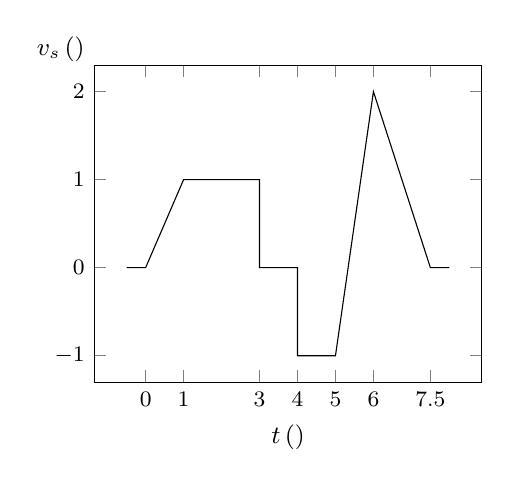
\begin{tikzpicture}
\begin{axis}[small,xlabel={$t\,(\si{\second})$},ylabel={$v_s\,(\si{\milli\volt})$},xtick={0,1,3,4,5,6,7.5},xticklabels={$0$,$1$,$3$,$4$,$5$,$6$,$7.5$},ytick={-1,0,1,2},yticklabels={$-1$,$0$,$1$,$2$},ylabel style={rotate=-90},ylabel style={at={(axis description cs:0,1.05)}}]
\addplot[] plot coordinates {(-0.5,0)(0,0) (1,1) (3,1) (3,0) (4,0) (4,-1) (5,-1) (6,2) (7.5,0) (8,0)};
\end{axis}
\end{tikzpicture}
\caption*{(الف)}
\end{subfigure}%
\begin{subfigure}{0.5\textwidth}
\centering
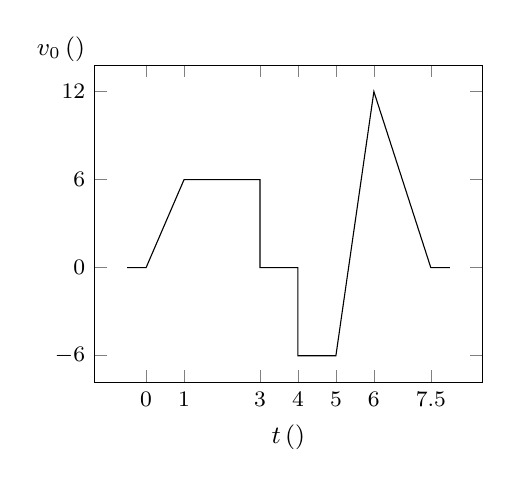
\begin{tikzpicture}
\begin{axis}[small,xlabel={$t\,(\si{\second})$},ylabel={$v_0\,(\si{\milli\volt})$},xtick={0,1,3,4,5,6,7.5},xticklabels={$0$,$1$,$3$,$4$,$5$,$6$,$7.5$},ytick={-1,0,1,2},yticklabels={$-6$,$0$,$6$,$12$},ylabel style={rotate=-90},ylabel style={at={(axis description cs:0,1.05)}}]
\addplot[] plot coordinates {(-0.5,0)(0,0) (1,1) (3,1) (3,0) (4,0) (4,-1) (5,-1) (6,2) (7.5,0) (8,0)};
\end{axis}
\end{tikzpicture}
\caption*{(ب)}
\end{subfigure}%
\caption{سوال \حوالہ{سوال_حسابی_داخلی_خارجی_اشارہ_الف} کے اشکال۔}
\label{شکل_سوال_حسابی_داخلی_خارجی_اشارہ_الف}
\end{figure}

جواب:شکل-ب
\انتہا{سوال}
%======================
\ابتدا{سوال}\شناخت{سوال_حسابی_داخلی_خارجی_اشارہ_ب}
ایک حسابی ایمپلیفائر کی افزائش \عددی{-10} ہے۔اس کا داخلی اشارہ شکل \حوالہ{شکل_سوال_حسابی_داخلی_خارجی_اشارہ_ب}-الف میں دیا گیا ہے۔خارجی اشارے کا خط کھینچیں۔
\begin{figure}
\centering
\begin{subfigure}{0.5\textwidth}
\centering
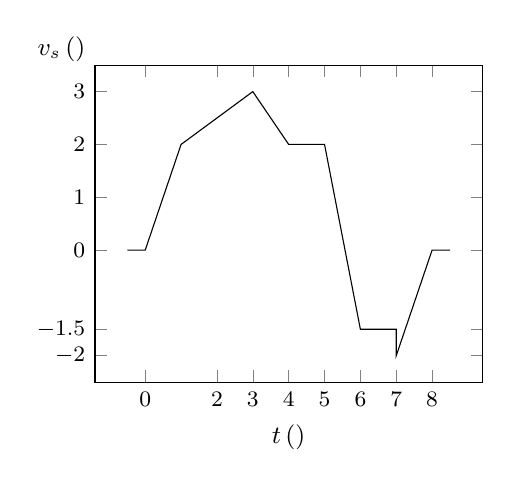
\begin{tikzpicture}
\begin{axis}[small,xlabel={$t\,(\si{\second})$},ylabel={$v_s\,(\si{\milli\volt})$},xtick={0,2,3,4,5,6,7,8},xticklabels={$0$,$2$,$3$,$4$,$5$,$6$,$7$,$8$},ytick={-2,-1.5,0,1,2,3},yticklabels={$-2$,$-1.5$,$0$,$1$,$2$,$3$},ylabel style={rotate=-90},ylabel style={at={(axis description cs:0,1.05)}}]
\addplot[] plot coordinates {(-0.5,0)(0,0)(1,2)(3,3)(4,2)(5,2)(6,-1.5)(7,-1.5)(7,-2) (8,0)(8.5,0)};
\end{axis}
\end{tikzpicture}
\caption*{(الف)}
\end{subfigure}%
\begin{subfigure}{0.5\textwidth}
\centering
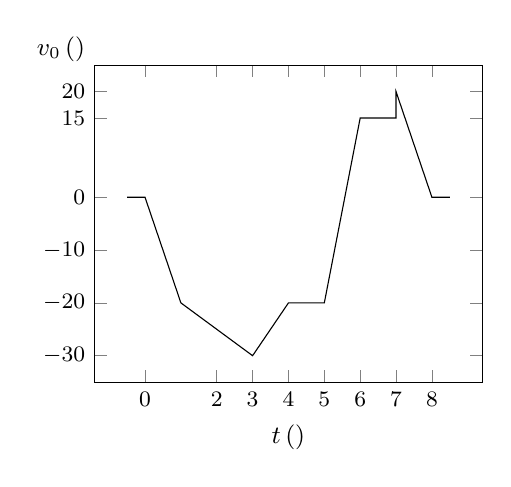
\begin{tikzpicture}
\begin{axis}[small,xlabel={$t\,(\si{\second})$},ylabel={$v_0\,(\si{\milli\volt})$},xtick={0,2,3,4,5,6,7,8},xticklabels={$0$,$2$,$3$,$4$,$5$,$6$,$7$,$8$},ytick={2,1.5,0,-1,-2,-3},yticklabels={$20$,$15$,$0$,$-10$,$-20$,$-30$},ylabel style={rotate=-90},ylabel style={at={(axis description cs:0,1.05)}}]
\addplot[] plot coordinates {(-0.5,0)(0,0)(1,-2)(3,-3)(4,-2)(5,-2)(6,1.5)(7,1.5)(7,2) (8,0)(8.5,0)};
\end{axis}
\end{tikzpicture}
\caption*{(ب)}
\end{subfigure}%
\caption{سوال \حوالہ{سوال_حسابی_داخلی_خارجی_اشارہ_ب} کے اشکال۔}
\label{شکل_سوال_حسابی_داخلی_خارجی_اشارہ_ب}
\end{figure}

جواب:شکل-ب
\انتہا{سوال}
%====================
\ابتدا{سوال}\شناخت{سوال_حسابی_داخلی_خارجی_اشارہ_پ}
ایک حسابی ایمپلیفائر کی افزائش \عددی{-20} ہے اور اس کو \عددی{\SI{\mp15}{\volt}} طاقت فراہم کی جا رہی ہے۔اس کا خارجی اشارہ شکل \حوالہ{شکل_سوال_حسابی_داخلی_خارجی_اشارہ_پ}-الف میں دیا گیا ہے۔داخلی اشارے کا خط کھینچیں۔
\begin{figure}
\centering
\begin{subfigure}{0.5\textwidth}
\centering
\begin{tikzpicture}
\begin{axis}[small,xlabel={$t\,(\si{\second})$},ylabel={$v_0\,(\si{\volt})$},xtick={0,4,6,7,9},xticklabels={$0$,$4$,$6$,$7$,$9$},ytick={-2,0,3},yticklabels={$-2$,$0$,$3$},ylabel style={rotate=-90},ylabel style={at={(axis description cs:0,1.05)}}]
\addplot[] plot coordinates {(0,0)(4,3)(6,-2)(7,-2)(10,1)};
\end{axis}
\end{tikzpicture}
\caption*{(الف)}
\end{subfigure}%
\begin{subfigure}{0.5\textwidth}
\centering
\begin{tikzpicture}
\begin{axis}[small,xlabel={$t\,(\si{\second})$},ylabel={$v_s\,(\si{\volt})$},xtick={0,1,3,4,5,6,7,9},xticklabels={$0$,$1$,$3$,$4$,$5$,$6$,$7$,$9$},ytick={-0.15,0,0.1},yticklabels={$-0.15$,$0$,$0.1$},ylabel style={rotate=-90},ylabel style={at={(axis description cs:0,1.05)}}]
\addplot[] plot coordinates {(0,0)(4,-0.15)(6,0.1)(7,0.1)(10,-0.05)};
\end{axis}
\end{tikzpicture}
\caption*{(ب)}
\end{subfigure}%
\caption{سوال \حوالہ{سوال_حسابی_داخلی_خارجی_اشارہ_پ} کے اشکال۔}
\label{شکل_سوال_حسابی_داخلی_خارجی_اشارہ_پ}
\end{figure}

جواب:شکل-ب
\انتہا{سوال}
%======================
\ابتدا{سوال}
کامل حسابی ایمپلیفائر کی داخلی مزاحمت لامتناہی اور خارجی مزاحمت صفر ہوتے ہیں۔ان کا داخلی رو اور داخلی دباو پر کیا اثر پایا جاتا ہے۔

حل:داخلی رو صفر ہوتی ہے۔ داخلی دباو صفر ہوتا ہے۔
\انتہا{سوال}
%=========================
\ابتدا{سوال}\شناخت{سوال_حسابی_ایمپلیفائر_الف}
شکل \حوالہ{شکل_سوال_حسابی_ایمپلیفائر_الف} کا افزائش دباو دریافت کریں اور \عددی{v_s=0.23\sin 10t\,\si{\volt}} کی صورت میں \عددی{v_0} حاصل کریں۔
\begin{figure}
\centering
\begin{tikzpicture}
\draw(0,0) node[op amp](u1){};
\draw(u1.+) to [short]++(-\x/8,0) node[ground]{};
\draw(u1.-) to [short]++(-\x/8,0) to [resistor,l_={$\SI{2.2}{\kilo\ohm}$}]++(-\x,0) ++(0,-\y) node[ground]{} to [american voltage source,l={$v_s$}]++(0,\y);
\draw(u1.-)++(-\x/8,0) to [short,*-] ++(0,\y/2) to [resistor,l={$\SI{14.7}{\kilo\ohm}$}]++(\x+\x/4,0)-|(u1.out);
\draw(u1.out) to [short,*-o]++(\x/2,0)node[right]{$v_0$};
\end{tikzpicture}
\caption{سوال \حوالہ{سوال_حسابی_ایمپلیفائر_الف} کا دور۔}
\label{شکل_سوال_حسابی_ایمپلیفائر_الف}
\end{figure}

جوابات:\عددی{A_v=\SI{-6.68}{\volt\per\volt}}، \عددی{v_0=-1.54\sin 10t\,\si{\volt}}
\انتہا{سوال}
%===========================
\ابتدا{سوال}\شناخت{سوال_حسابی_ایمپلیفائر_ب}
شکل \حوالہ{شکل_سوال_حسابی_ایمپلیفائر_ب} کا افزائش دباو دریافت کریں اور \عددی{v_s=0.16\cos 314t\,\si{\volt}} کی صورت میں \عددی{v_0} حاصل کریں۔
\begin{figure}
\centering
\begin{tikzpicture}
\draw(0,0) node[op amp](u1){};
\draw(u1.+) to [short]++(-\x/8,0)++(0,-\y)  node[ground]{} to [american voltage source,l={$v_s$}]++(0,\y);
\draw(u1.-) to [short]++(-\x/8,0) to [resistor,l_={$\SI{1.8}{\kilo\ohm}$}]++(-\x,0) node[ground]{};
\draw(u1.-)++(-\x/8,0) to [short,*-] ++(0,\y/2) to [resistor,l={$\SI{22}{\kilo\ohm}$}]++(\x+\x/4,0)-|(u1.out);
\draw(u1.out) to [short,*-o]++(\x/2,0)node[right]{$v_0$};
\end{tikzpicture}
\caption{سوال \حوالہ{سوال_حسابی_ایمپلیفائر_ب} کا دور۔}
\label{شکل_سوال_حسابی_ایمپلیفائر_ب}
\end{figure}

جوابات:\عددی{A_v=\SI{13.22}{\volt\per\volt}}، \عددی{v_0=2.12\cos 314t\,\si{\volt}}
\انتہا{سوال}
%===========================
\ابتدا{سوال}\شناخت{سوال_حسابی_ایمپلیفائر_پ}
شکل \حوالہ{شکل_سوال_حسابی_ایمپلیفائر_پ} کا افزائش دباو دریافت کریں۔
\begin{figure}
\centering
\begin{tikzpicture}
\draw(0,0) node[op amp](u1){};
\draw(u1.+) to [short]++(-\x/8,0)++(0,-\y)  node[ground]{} to [resistor,l_={$\SI{10}{\kilo\ohm}$}]++(0,\y) to [resistor,*-,l={$\SI{40}{\kilo\ohm}$}]++(-\x,0)++(0,-\y) node[ground]{} to [american voltage source,l={$v_s$}]++(0,\y);
\draw(u1.-) to [short]++(-\x/8,0) to [resistor,l_={$\SI{2}{\kilo\ohm}$}]++(-\x,0) node[ground]{};
\draw(u1.-)++(-\x/8,0) to [short,*-] ++(0,\y/2) to [resistor,l={$\SI{48}{\kilo\ohm}$}]++(\x+\x/4,0)-|(u1.out);
\draw(u1.out) to [short,*-o]++(\x/2,0)node[right]{$v_0$};
\end{tikzpicture}
\caption{سوال \حوالہ{سوال_حسابی_ایمپلیفائر_پ} کا دور۔}
\label{شکل_سوال_حسابی_ایمپلیفائر_پ}
\end{figure}

جوابات:\عددی{A_v=\SI{5}{\volt\per\volt}}
\انتہا{سوال}
%===========================
\ابتدا{سوال}\شناخت{سوال_حسابی_ایمپلیفائر_ت}
شکل \حوالہ{شکل_سوال_حسابی_ایمپلیفائر_ت} کا افزائش دباو دریافت کریں۔کامل حسابی ایمپلیفائر استعمال کیا گیا ہے۔
\begin{figure}
\centering
\begin{tikzpicture}
\draw(0,0) node[op amp,yscale=-1](u1){};
\draw(u1.+) to [short]++(-\x/8,0) to [resistor,-o,l_={$\SI{2}{\kilo\ohm}$}]++(-\x,0)node[left]{$v_s$};
\draw(u1.out) to [resistor,-*,l={$R_2$}]++(0,-\y)coordinate(kM) to [resistor,l={$R_1$}]++(0,-\y) node[ground]{};
\draw(u1.-) |-(kM);
\draw(u1.out) to [short,*-o]++(\x/2,0)node[right]{$v_0$};
\end{tikzpicture}
\caption{سوال \حوالہ{سوال_حسابی_ایمپلیفائر_ت} کا دور۔}
\label{شکل_سوال_حسابی_ایمپلیفائر_ت}
\end{figure}

جوابات:داخلی جانب نسب \عددی{\SI{2}{\kilo\ohm}} کا افزائش پر کوئی اثر نہیں پایا جاتا لہٰذا \عددی{A_v=1+\tfrac{R_2}{R_1}} ہے۔
\انتہا{سوال}
%===========================
\ابتدا{سوال}\شناخت{سوال_حسابی_ایمپلیفائر_ٹ}
شکل \حوالہ{شکل_سوال_حسابی_ایمپلیفائر_ٹ} کا افزائش دباو دریافت کریں۔داخلی دباو \عددی{v_s=\SI{0.4}{\volt}} کی صورت میں \عددی{I_0} دریافت کریں۔
\begin{figure}
\centering
\begin{tikzpicture}
\draw(0,0) node[op amp](u1){};
\draw(u1.+) to [short]++(-\x/8,0) node[ground]{};
\draw(u1.-) to [short]++(-\x/2,0) to [resistor,l_={$\SI{12}{\kilo\ohm}$}]++(-\x,0) ++(0,-\y) node[ground]{} to [american voltage source,l={$v_s$}]++(0,\y);
\draw(u1.-)++(-\x/2,0) to [short,*-] ++(0,\y/2) to [resistor,l={$\SI{82}{\kilo\ohm}$}]++(\x+\x/4,0)-|(u1.out);
\draw(u1.-)++(-\x/2,0) to [resistor,l_={$\SI{10}{\kilo\ohm}$}]++(0,-\y)node[ground]{};
\draw(u1.out) to [short,*-o]++(\x/2,0)node[right]{$v_0$};
\draw(u1.out) to [resistor,l={$\SI{5}{\kilo\ohm}$},i={$I_0$}]++(0,-\y)node[ground]{};
\end{tikzpicture}
\caption{سوال \حوالہ{سوال_حسابی_ایمپلیفائر_ٹ} کا دور۔}
\label{شکل_سوال_حسابی_ایمپلیفائر_ٹ}
\end{figure}

جوابات:\عددی{A_v=-\tfrac{41}{6}\,\si{\volt\per\volt}}، \عددی{I_0=-\tfrac{41}{75}\,\si{\milli\ampere}}
\انتہا{سوال}
%===========================
\ابتدا{سوال}\شناخت{سوال_حسابی_ایمپلیفائر_ث}
شکل \حوالہ{شکل_سوال_حسابی_ایمپلیفائر_ث} کا افزائش دباو دریافت کریں۔
\begin{figure}
\centering
\begin{tikzpicture}
\draw(0,0) node[op amp](u1){};
\draw(u1.+) to [short]++(-\x/8,0) node[ground]{};
\draw(u1.-) to [short]++(-\x/2,0) to [resistor,l_={$\SI{12}{\kilo\ohm}$}]++(-\x,0) to [resistor,l_={$\SI{8}{\kilo\ohm}$}]++(-\x,0) ++(0,-\y) node[ground]{} to [american voltage source,l={$v_s$}]++(0,\y);
\draw(u1.-)++(-\x/2,0) to [short,*-] ++(0,\y/2)coordinate(kUL) to [resistor,l={$\SI{82}{\kilo\ohm}$}]++(\x+\x/4,0)-|(u1.out);
%
\path[name path={kvert}](u1.out)--++(0,\y);
\path[name path={khort}](kUL)++(\x+\x/4,0)--++(\x,0);
%
\draw[name intersections={of=kvert and khort}](kUL) to [short,*-]++(0,\y/2) to [resistor,l={$\SI{36}{\kilo\ohm}$}]++(\x+\x/4,0)-|(intersection-1)node[circ]{};
\draw(u1.-)++(-\x/2,0) to [resistor,l_={$\SI{10}{\kilo\ohm}$}]++(0,-\y)node[ground]{};
\draw(u1.out) to [short,*-o]++(\x/2,0)node[right]{$v_0$};
\draw(u1.out) to [resistor,l={$\SI{5}{\kilo\ohm}$}]++(0,-\y)node[ground]{};
\end{tikzpicture}
\caption{سوال \حوالہ{سوال_حسابی_ایمپلیفائر_ث} کا دور۔}
\label{شکل_سوال_حسابی_ایمپلیفائر_ث}
\end{figure}

جوابات:\عددی{A_v=-\tfrac{369}{295}\,\si{\volt\per\volt}}
\انتہا{سوال}
%===========================
\ابتدا{سوال}\شناخت{سوال_حسابی_ایمپلیفائر_ج}
شکل \حوالہ{شکل_سوال_حسابی_ایمپلیفائر_ج} میں کامل حسابی ایمپلیفائر استعمال کیا گیا ہے۔اس میں \عددی{I_1} اور \عددی{I_2} حاصل کریں۔
\begin{figure}
\centering
\begin{tikzpicture}
\draw(0,0) node[op amp,yscale=-1](u1){};
\draw(u1.+) to [short,-o,i^<={$I_1$}]++(-\x/2,0)node[left]{$\SI{-2}{\volt}$};
\draw(u1.out) to [short,*-o]++(\x/2,0)node[right]{$v_0$};
\draw(u1.-) to [short,-*]++(0,-\y/2)coordinate(kL) to [resistor,l_={$\SI{2}{\kilo\ohm}$}]++(0,-\y)node[ground]{};
\draw(kL) to [resistor,l_={$\SI{8}{\kilo\ohm}$},i<={$I_2$}]++(\x,0)-|(u1.out);
\end{tikzpicture}
\caption{سوال \حوالہ{سوال_حسابی_ایمپلیفائر_ج} کا دور۔}
\label{شکل_سوال_حسابی_ایمپلیفائر_ج}
\end{figure}

جوابات:\عددی{I_1=0}، \عددی{I_2=\SI{-1}{\milli\ampere}}
\انتہا{سوال}
%===========================
\ابتدا{سوال}\شناخت{سوال_حسابی_ایمپلیفائر_دیگر_الف}
شکل \حوالہ{شکل_سوال_حسابی_ایمپلیفائر_دیگر_الف} کا حسابی ایمپلیفائر \عددی{\SI{60}{\milli\ampere}} سے زیادہ رو مہیا نہیں کر سکتا۔ایمپلیفائر کو \عددی{\SI{\mp 18}{\volt}} سے طاقت فراہم کی گئی ہے۔اس کی افزائش \عددی{R_1} اور \عددی{R_2} سے اس طرح تعین کی جاتی ہے کہ \عددی{R_1+R_2=\SI{20}{\kilo\ohm}} رہے۔زیادہ سے زیادہ ممکنہ افزائش کیا ممکن ہے۔
\begin{figure}
\centering
\begin{tikzpicture}
\draw(0,0) node[op amp](u1){};
\draw(u1.+) to [short]++(-\x/8,0) node[ground]{};
\draw(u1.-) to [short]++(-\x/8,0) to [resistor,l_={$R_1$}]++(-\x,0) ++(0,-\y) node[ground]{} to [american voltage source,l={$\SI{0.24}{\volt}$}]++(0,\y);
\draw(u1.-)++(-\x/8,0) to [short,*-] ++(0,\y/2) to [resistor,l={$R_2$}]++(\x+\x/4,0)-|(u1.out);
\draw(u1.out) to [short,*-o]++(\x/2,0)node[right]{$v_0$};
\draw(u1.out) to [resistor,l={$\SI{200}{\ohm}$}]++(0,-\y) node[ground]{};
\end{tikzpicture}
\caption{سوال \حوالہ{سوال_حسابی_ایمپلیفائر_دیگر_الف} کا دور۔}
\label{شکل_سوال_حسابی_ایمپلیفائر_دیگر_الف}
\end{figure}

جوابات:\عددی{A_v=\SI{-50}{\volt\per\volt}}
\انتہا{سوال}
%========================
\ابتدا{سوال}\شناخت{سوال_حسابی_ایمپلیفائر_دیگر_ب}
شکل \حوالہ{شکل_سوال_حسابی_ایمپلیفائر_دیگر_ب} رو سے دباو حاصل کرتا ہے۔خارجی دباو \عددی{v_0} حاصل کریں۔بیرونی بوجھ مزاحمت کی رو \عددی{I_0} بھی حاصل کریں۔
\begin{figure}
\centering
\begin{tikzpicture}
\draw(0,0) node[op amp](u1){};
\draw(u1.+) to [short]++(-\x/8,0) node[ground]{};
\draw(u1.-) to [short]++(-\x/8,0) to [short]++(-\x,0) ++(0,-\y) node[ground]{} to [american current source,l={$\SI{2}{\milli\ampere}$}]++(0,\y);
\draw(u1.-)++(-\x/8,0) to [short,*-] ++(0,\y/2) to [resistor,l={$\SI{4}{\kilo\ohm}$}]++(\x+\x/4,0)-|(u1.out);
\draw(u1.out) to [short,*-o]++(\x/2,0)node[right]{$v_0$};
\draw(u1.out) to [resistor,l={$\SI{80}{\ohm}$},i={$I_0$}]++(0,-\y) node[ground]{};
\end{tikzpicture}
\caption{سوال \حوالہ{سوال_حسابی_ایمپلیفائر_دیگر_ب} کا دور۔}
\label{شکل_سوال_حسابی_ایمپلیفائر_دیگر_ب}
\end{figure}

جوابات:\عددی{v_0=\SI{-8}{\volt}}، \عددی{I_0=\SI{-100}{\milli\ampere}}
\انتہا{سوال}
%========================
\ابتدا{سوال}\شناخت{سوال_حسابی_ایمپلیفائر_دیگر_پ}
شکل \حوالہ{شکل_سوال_حسابی_ایمپلیفائر_دیگر_پ} میں موصل نما افزائش \عددی{\tfrac{I_0}{V_s}} دریافت کریں۔
\begin{figure}
\centering
\begin{tikzpicture}
\draw(0,0) node[op amp](u1){};
\draw(u1.+) to [short]++(-\x/8,0) ++(0,-\y) node[ground]{} to [american voltage source,l={$V_s$}]++(0,\y);
\draw(u1.-) to [short]++(-\x/8,0) to [resistor,l_={$\SI{2}{\kilo\ohm}$}]++(-\x,0) node[ground]{};
\draw(u1.-)++(-\x/8,0) to [short,*-] ++(0,\y/2) to [resistor,l={$\SI{6}{\kilo\ohm}$},i<={$I_0$}]++(\x+\x/4,0)-|(u1.out);
\end{tikzpicture}
\caption{سوال \حوالہ{سوال_حسابی_ایمپلیفائر_دیگر_پ} کا دور۔}
\label{شکل_سوال_حسابی_ایمپلیفائر_دیگر_پ}
\end{figure}

جوابات:\عددی{\tfrac{I_0}{V_s}=\tfrac{1}{2}\,\si{\milli\ampere\per\volt}}
\انتہا{سوال}
%========================
\ابتدا{سوال}\شناخت{سوال_حسابی_ایمپلیفائر_دیگر_ت}
شکل \حوالہ{شکل_سوال_حسابی_ایمپلیفائر_دیگر_ت} میں خارجی دباو \عددی{v_0} دریافت کریں۔
\begin{figure}
\centering
\begin{tikzpicture}
\draw(0,0) node[op amp](u1){};
\draw(u1.+) to [short]++(-\x/8,0) ++(0,-\y) node[ground]{} to [american voltage source,l={$\SI{2.2}{\volt}$}]++(0,\y);
\draw(u1.-) to [short]++(-\x/8,0) to [resistor,l_={$\SI{800}{\ohm}$}]++(-\x,0) ++(0,-\y) node[ground]{} to [american voltage source,l={$\SI{2}{\volt}$}]++(0,\y);
\draw(u1.-)++(-\x/8,0) to [short,*-] ++(0,\y/2) to [resistor,l={$\SI{12}{\kilo\ohm}$}]++(\x+\x/4,0)-|(u1.out);
\draw(u1.out) to [short,*-o]++(\x/4,0)node[right]{$v_0$};
\end{tikzpicture}
\caption{سوال \حوالہ{سوال_حسابی_ایمپلیفائر_دیگر_ت} کا دور۔}
\label{شکل_سوال_حسابی_ایمپلیفائر_دیگر_ت}
\end{figure}

جوابات:\عددی{v_0=\SI{5.2}{\volt}}
\انتہا{سوال}
%========================
\ابتدا{سوال}\شناخت{سوال_حسابی_ایمپلیفائر_دیگر_ٹ}
شکل \حوالہ{شکل_سوال_حسابی_ایمپلیفائر_دیگر_ٹ} میں خارجی دباو \عددی{v_0} اور داخلی دباو \عددی{v_1}، \عددی{v_2} کا تعلق دریافت کریں۔
\begin{figure}
\centering
\begin{tikzpicture}
\draw(0,0) node[op amp](u1){};
\draw(u1.+) to [short]++(-\x/8,0) ++(0,-\y) node[ground]{} to [american voltage source,l={$v_2$}]++(0,\y);
\draw(u1.-) to [short]++(-\x/8,0) to [resistor,l_={$R_1$}]++(-\x,0) ++(0,-\y) node[ground]{} to [american voltage source,l={$v_1$}]++(0,\y);
\draw(u1.-)++(-\x/8,0) to [short,*-] ++(0,\y/2) to [resistor,l={$R_2$}]++(\x+\x/4,0)-|(u1.out);
\draw(u1.out) to [short,*-o]++(\x/4,0)node[right]{$v_0$};
\end{tikzpicture}
\caption{سوال \حوالہ{سوال_حسابی_ایمپلیفائر_دیگر_ٹ} کا دور۔}
\label{شکل_سوال_حسابی_ایمپلیفائر_دیگر_ٹ}
\end{figure}

جوابات:\عددی{v_0=(1+\tfrac{R_2}{R_1})v_2-\tfrac{R_2}{R_1}v_1}
\انتہا{سوال}
%========================
\ابتدا{سوال}\شناخت{سوال_حسابی_ایمپلیفائر_دیگر_ث}
شکل \حوالہ{شکل_سوال_حسابی_ایمپلیفائر_دیگر_ث} میں خارجی دباو \عددی{v_0} اور داخلی دباو \عددی{v_1}، \عددی{v_2} کا تعلق دریافت کریں۔
\begin{figure}
\centering
\begin{tikzpicture}
\draw(0,0) node[op amp](u1){};
\draw(u1.+) to [short]++(-\x/8,0)coordinate(kUL) to [resistor,l={$R_4$}]++(0,-\y)node[ground]{};
\draw(kUL) to [resistor,*-o,l={$R_3$}]++(-\x,0)node[left]{$v_2$};
\draw(u1.-) to [short]++(-\x/8,0) to [resistor,-o,l_={$R_1$}]++(-\x,0)node[left]{$v_1$};
\draw(u1.-)++(-\x/8,0) to [short,*-] ++(0,\y/2) to [resistor,l={$R_2$}]++(\x+\x/4,0)-|(u1.out);
\draw(u1.out) to [short,*-o]++(\x/4,0)node[right]{$v_0$};
\end{tikzpicture}
\caption{سوال \حوالہ{سوال_حسابی_ایمپلیفائر_دیگر_ث} کا دور۔}
\label{شکل_سوال_حسابی_ایمپلیفائر_دیگر_ث}
\end{figure}

جوابات:\عددی{v_0=(\tfrac{R_1+R_2}{R_3+R_4})(\tfrac{R_4}{R_1})v_2-\tfrac{R2}{R1}v_1}
\انتہا{سوال}
%========================
\ابتدا{سوال}\شناخت{سوال_حسابی_مشکل_الف}
شکل \حوالہ{شکل_سوال_حسابی_مشکل_الف} میں \عددی{v_0} حاصل کریں۔ 
\begin{figure}
\centering
\begin{tikzpicture}
\draw(0,0)node[op amp](u1){};
\draw(u1.+) to [short]++(-\x/8,0)node[ground]{};
\draw(u1.-)to [short,-*]++(-\x/8,0)coordinate(kR) to [short,-*]++(-\x/4,0)coordinate(kL);
\draw(kR) to [short]++(0,\y/2) to [resistor,l={$R_0$}]++(\x+\x/4,0)-|(u1.out);
\draw(u1.out) to [short,*-o]++(\x/4,0)node[right]{$v_0$};
\draw(kL)  to [short] ++(0,\y/2) to [resistor,-o,l_={$R_1$}]++(-\x,0)node[left]{$v_1$};
\draw(kL) to [resistor,-o,l_={$R_2$}]++(-\x,0)node[left]{$v_2$};
\draw(kL) to [short] ++(0,-\y/2) to [resistor,-o,l_={$R_3$}]++(-\x,0)node[left]{$v_3$};
\end{tikzpicture}
\caption{سوال \حوالہ{سوال_حسابی_مشکل_الف} کا دور۔}
\label{شکل_سوال_حسابی_مشکل_الف}
\end{figure}

جواب:\عددی{v_0=-R_0(\tfrac{v_1}{R_1}+\tfrac{v_2}{R_2}+\tfrac{v_3}{R_3})}
\انتہا{سوال}
%====================================
\ابتدا{سوال}\شناخت{سوال_حسابی_مشکل_ب}
شکل \حوالہ{شکل_سوال_حسابی_مشکل_ب} میں \عددی{v_0} حاصل کریں۔ 
\begin{figure}
\centering
\begin{tikzpicture}
\draw(0,0)node[op amp,yscale=-1](u1){};
\draw(u1.+)to [short,-*]++(-\x/2,0)coordinate(kL);
\draw(u1.out) to [short,*-o]++(\x/4,0)node[right]{$v_0$};
\draw(kL)  to [short] ++(0,\y) to [resistor,-o,l_={$R_1$}]++(-\x,0)node[left]{$v_1$};
\draw(kL) to [short] ++(0,\y/2) to [resistor,*-o,l_={$R_2$}]++(-\x,0)node[left]{$v_2$};
\draw(kL)  to [resistor,-o,l_={$R_3$}]++(-\x,0)node[left]{$v_3$};
\draw(u1.-) to [short]++(-\x/8,0) to [short]++(0,-\y/2) to [resistor,l={$R_5$}]++(\x+\x/4,0)-|(u1.out);
\draw(u1.-)++(-\x/8,0) to [resistor,*-,l={$R_4$}]++(-\x,0)node[ground]{};
\end{tikzpicture}
\caption{سوال \حوالہ{سوال_حسابی_مشکل_ب} کا دور۔}
\label{شکل_سوال_حسابی_مشکل_ب}
\end{figure}

جواب:
$v_0=\frac{1+\frac{R_5}{R_4}}{\frac{1}{R_1}+\frac{1}{R_2}+\frac{1}{R_3}} \left[\frac{v_1}{R_1}+\frac{v_2}{R_2}+\frac{v_3}{R_3}\right]$
\انتہا{سوال}
%====================
\ابتدا{سوال}\شناخت{سوال_حسابی_مشکل_پ}
شکل \حوالہ{شکل_سوال_حسابی_مشکل_پ} میں \عددی{v_{01}} اور \عددی{v_1} کا تعلق دریافت کریں۔اب \عددی{v_{02}} کا \عددی{v_2} اور \عددی{v_{01}} کے ساتھ تعلق دریافت کریں۔ان نتائج کو استعمال کرتے ہوئے \عددی{v_{02}} کا \عددی{v_1} اور \عددی{v_2} کے ساتھ تعلق لکھیں۔
\begin{figure}
\centering
\begin{tikzpicture}
\draw(0,0)node[op amp](u1){};
\draw(2*\x+\x/2,-\y/3) node[op amp](u2){};
\draw(u1.+) to [short]++(-\x/8,0)node[ground]{};
\draw(u1.-) to [resistor,-o,l_={$R_1$}]++(-\x,0)node[left]{$v_1$};
\draw(u1.-) to [short,*-]++(0,\y/2) to [resistor,l={$R_2$}]++(\x,0)-|(u1.out);
\draw(u1.out)node[above right]{$v_{01}$};
\draw(u2.-) to [resistor,l_={$R_3$}]++(-\x,0)-|(u1.out);
\draw(u2.+) to [short,-o]++(-\x/4,0)node[left]{$v_2$};
\draw(u2.-) to [short,*-]++(0,\y/2) to [resistor,l={$R_4$}]++(\x,0)-|(u2.out);
\draw(u2.out) to [short,*-o]++(\x/4,0)node[right]{$v_{02}$};
\draw(u1.out)node[circ]{};
\end{tikzpicture}
\caption{سوال \حوالہ{سوال_حسابی_مشکل_پ} کا دور۔}
\label{شکل_سوال_حسابی_مشکل_پ}
\end{figure}

جوابات:
\begin{align*}
v_{01}&=-\frac{R_2}{R_1}v_1\\
v_{02}&=\left(1+\frac{R_4}{R_3}\right)v_2-\frac{R_4}{R_3}v_{01}\\
v_{02}&=\left(1+\frac{R_4}{R_3}\right)v_2+\frac{R_4 R_2}{R_3 R_1}v_1
\end{align*}
\انتہا{سوال}
%======================
